\chapter{决策和意识} \label{chap:chap56}

在前面的章节中,我们已经了解了感官输入如何转化为神经活动,然后由大脑进行处理以产生即时知觉,以及这些知觉如何存储为短期和长期记忆(第~\ref{chap:chap52}~至~\ref{chap:chap54}~章)。
我们还详细检查了脊髓和大脑如何控制运动。
在这里,我们开始考虑神经科学最具挑战性的方面之一:通过决策的高阶认知过程将感觉输入转化为运动输出。
通过这一过程,我们得以一窥高级思维和意识的基本构成要素。


在神经科学之外,术语认知通常意味着与反射和专用例程有一些区别,但正如我们将看到的,神经科学在简单的行为中认识到认知的基本原理,这些简单的行为表现出两种类型的灵活性:偶然性和不受即时性的影响。
偶然性意味着刺激不会像反射时那样命令或启动动作。
刺激可能会激发特定的行为,但该行动可能会延迟,等待其他信息,或者可能永远不会发生。
这种免于即时行动的自由意味着有些操作会随着时间的推移而发生,这些操作不会立即受到环境变化或身体控制的实时需求的影响。


当我们做决定时,两种类型的灵活性(应急性和时间性)都会体现出来。
当然,并不是所有的决定都会调用认知。
许多行为例程(游泳、步行、喂食和梳理)都有可以称为决定的分支点,但它们以有序的方式进行,没有太多的灵活性或节奏控制。
它们主要受神经传递的时间步长支配,并且大部分专用于特定的输入-输出关系。
做出这些区分的目的不是要围绕决策制定明确的界限,而是要帮助我们关注决策的各个方面,使其成为认知模型。


出于目前的目的,我们将使用以下定义:决策是基于证据(感官输入)、先验知识(记忆)和预期结果对提议、行动或计划的承诺。
该承诺是临时的。
它不需要行为,并且可以修改。
我们可以改变主意。
关键的组成部分是对证据的某些考虑会导致有机体状态发生变化,我们将其比作行动、策略或新心理过程的临时实施。


这样的提议可以表示为一个行动计划:我决定向右转,离开安全的避难所,寻找水源,选择一条最不可能遇到捕食者的路径,接近一个陌生人,或者在 一本书。
计划的概念强调免于即时性。
此外,并非所有计划都会实现。 并非所有的思想都会导致行动,但将思想视为一种行动计划是有用的。
这种观点让我们把知晓看作是定向的(主要是无意识的)询问的结果,而不是神经表征的涌现特性。


决策已经在结构简单的生物中进行了研究,尤其是蠕虫、苍蝇、蜜蜂和水蛭,以及从老鼠到灵长类动物的哺乳动物。
较简单的生物之所以具有吸引力,是因为它们的神经系统较小,但它们缺乏研究需要认知形式的决策所需的行为库。
希望这些物种的生物学见解能够帮助我们理解哺乳动物,尤其是灵长类动物的特征过程。
这是一个值得称赞的目标,因为正如柏拉图所说,决策提供了我们精确划分认知功能的最佳机会,即确定支持其正常功能的共同原则,并阐明它们的机制,以便它们可以在疾病中得到修复。


在本章中,我们主要关注灵长类动物在人为设置下做出的感知决定。
这些原则自然地扩展到基于证据的推理和根据价值偏好做出的决策。
在本章的最后一部分,我们对认知的更广泛方面进行了深入了解。
从决策的角度来看,与知道和有意识地意识到相关的大脑状态可能比通常认为的更接近神经生物学解释。



\section{感知的鉴别需要一个决策规则}

直到最近,决策制定主要由经济学家和政治学家研究。
然而,在感知领域工作的心理学家和神经科学家长期以来一直关注决策。
事实上,最简单的决策类型涉及对微弱刺激的检测,例如昏暗的光线或微弱的声音、气味或触摸。
受试者必须决定刺激是否存在,即判断为“是”或“否”。
在实验室中,刺激可能出现的地点和时间具有很高的确定性。
因此,此类实验被用于从行为推断感觉系统的基本敏感性,行为是心理学的一个子领域,称为心理物理学。
检测实验在推断感应轻触、微弱声音和昏暗灯光的感觉神经元的信噪比特性方面发挥了作用。
在最后一种情况下,此类实验提供了证据,表明视觉系统能够检测到受光感受器背景噪声影响的最暗光,即单个光子。
换句话说,根据物理定律,它是尽可能高效的。


对知觉的心理物理学研究始于 19 世纪的\textit{能斯特$\cdot$韦伯}和\textit{古斯塔夫$\cdot$费希纳}。
他们感兴趣的是测量两种感官刺激之间可检测到的最小强度差异。
这样的测量可以揭示感觉处理的基本原理,而无需从神经元进行记录。
事实证明,它们也为决策的神经科学奠定了基础,因为每个是/否答案都是基于感官证据的选择。


在第~\ref{chap:chap17}~章中,我们了解了心理物理学家如何概念化检测问题(方框~\ref{box:17_1})。
在任何一项试验中,世界的状态要么是存在刺激,要么是没有刺激。
该决定基于含有噪声的证据样本。
如果存在刺激,则证据是从信号+噪声的概率分布中抽取的随机样本。
如果没有刺激,则证据是来自仅噪声分布的样本(图~\ref{fig:56_1}A)。
大脑并不直接感知刺激,而是接收样本的神经表征。
因此,一些噪音来自于形成这种表征所涉及的神经活动。
大脑的工作是使用以神经放电率编码的信息来决定样本来自哪个分布。
然而,大脑无法访问这些分布,只能访问每个给定决策中涉及的一个样本。
正是这些分布的分离(它们不重叠的程度)决定了刺激与噪声的可辨别性。
如果证据超过某些标准或阈值,则决策规则是说“是”。


\begin{figure}[htbp]
	\centering
	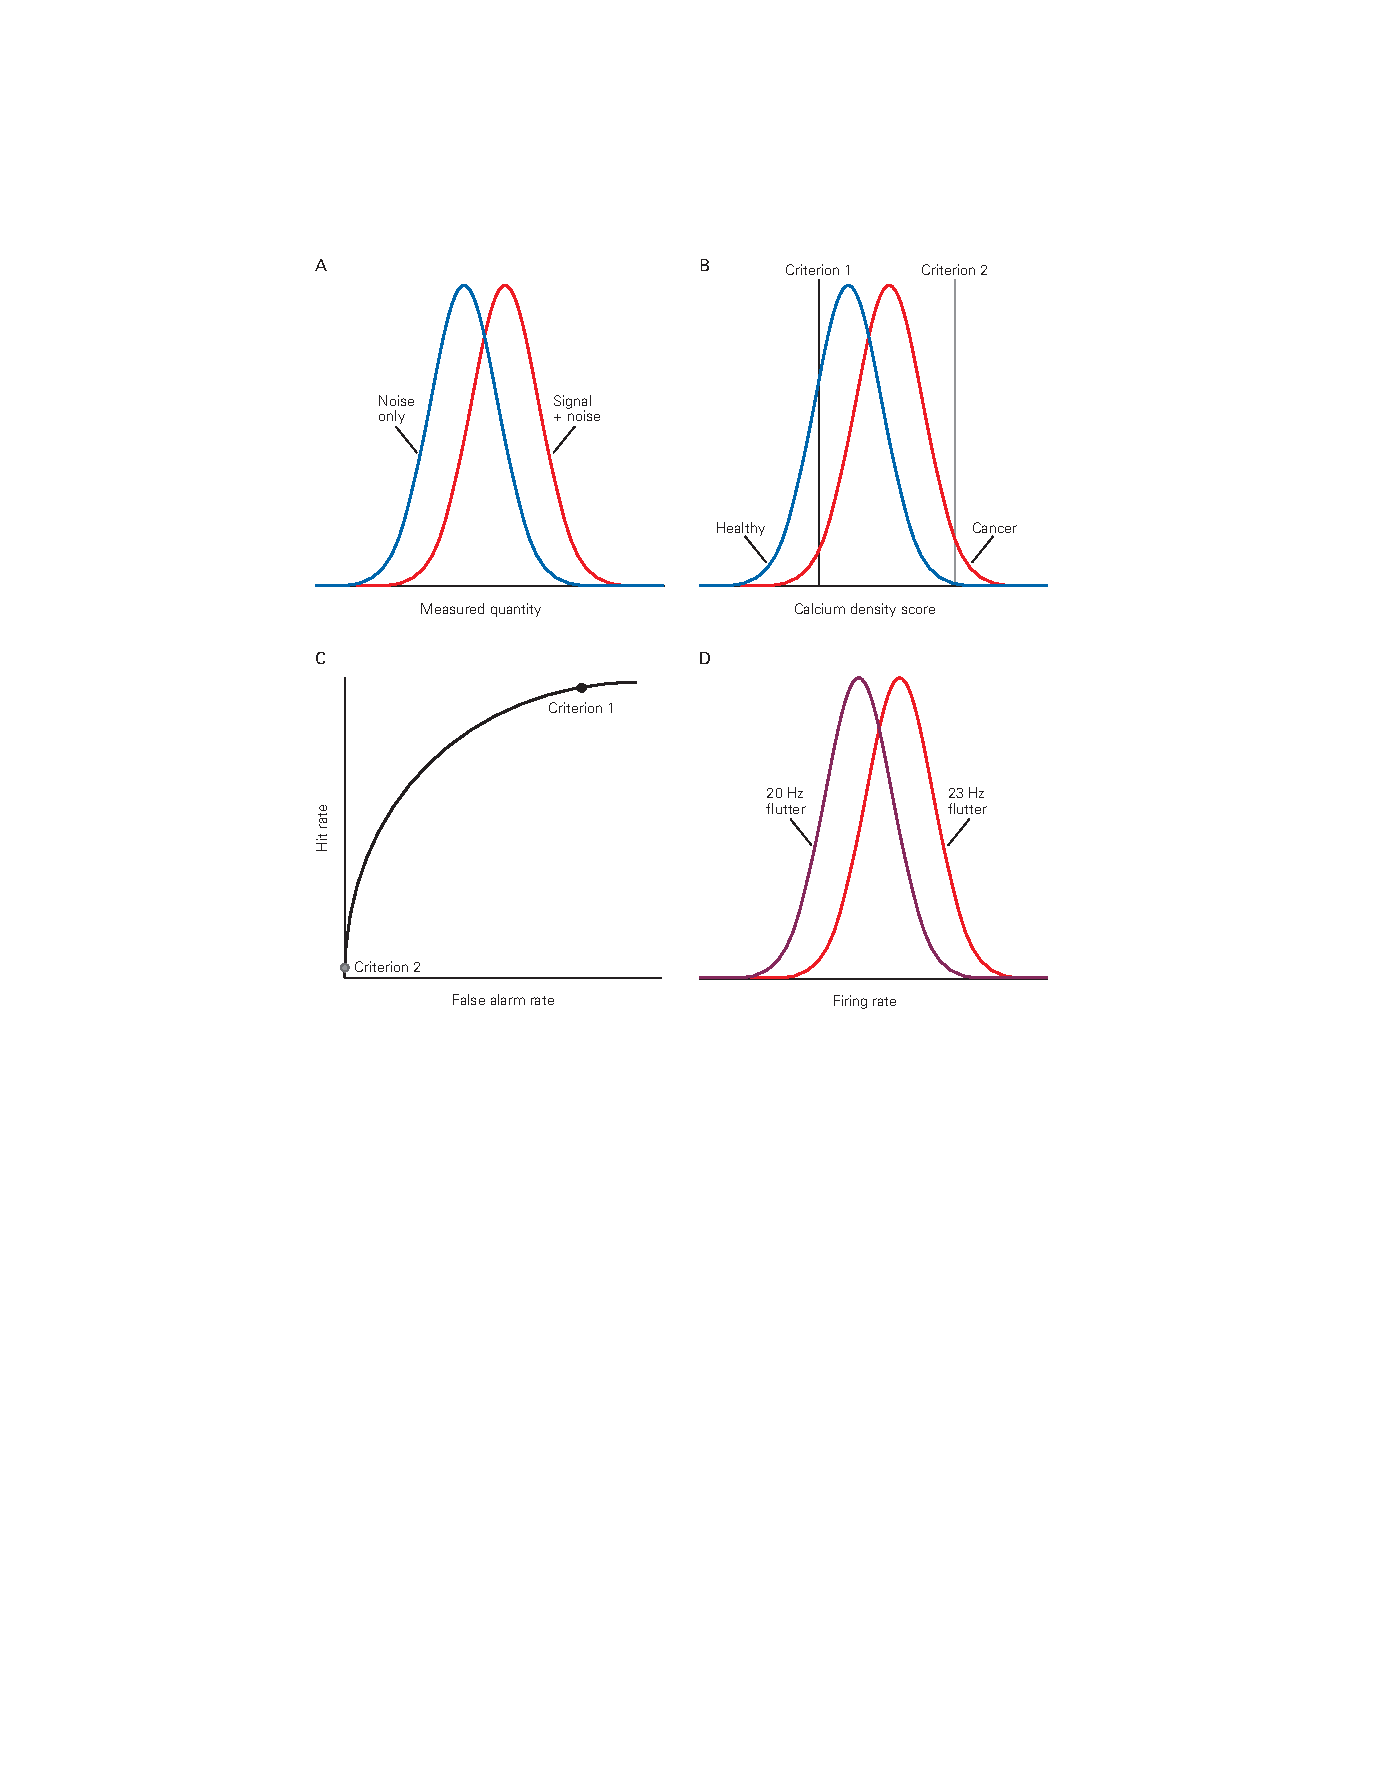
\includegraphics[width=0.97\linewidth]{chap56/fig_56_1}
	\caption{信号检测理论的框架形式化了证据和决策之间的关系。
		在面板 A 到 C 中,我们考虑简单的是-否决策,决策者只接受一个测量值。
		\textbf{A.} 曲线的高度表示在信号存在或不存在两种情况下观察到 x 轴测量值(每秒尖峰数、放射性计数或血压)的概率。
		在这两种情况下,测量都是可变的,从而导致与这两种情况相关的可能值的分布。
		如果存在信号,则决策者会从信号 + 噪声概率分布(红色)中接收随机样本。
		如果信号不存在,决策者会从仅噪声概率分布(蓝色)中接收样本。
		通过将测量值与标准或阈值进行比较,并回答是或否,信号存在或不存在(如果值大于或小于标准)来做出决定。
		\textbf{B.} 标准是政策的表达,如医疗决策中所说明的那样。 假设该度量是从筛查乳房 X 线照片中检测到的钙化点得出的:一个结合了数量、密度和形状的分数。
		将测试解释为阳性或阴性(是否患有乳腺癌)的标准 1(左线)是自由的。
		它会导致许多假阳性(83\%),但很少有癌症女性会得到阴性结果。
		标准 2(右线)是保守的。
		它会错过许多癌症病例,但它很少会给健康人带来积极的结果。
		如果一个积极的决定是危险(或痛苦)程序的理由,那将是有道理的。
		\textbf{C.} 接收器操作特性显示了所有可能标准的正确(命中率)和不正确(误报率)的“是”决定的比例组合。 自由主义和保守主义标准分别由黑色和灰色符号表示。
		\textbf{D.} 该框架也适用于两个备选方案之间的决策。
		这里,决定是施加到食指的振动是否比几秒前施加的振动具有更高的频率。
		重叠分布的相同描述可能符合代表感官刺激的大脑某些部分的神经反应。
		例如,体感皮层中的神经元可能会在许多单独的试验中对 23 赫兹的手指振动刺激的平均尖峰率高于 20 赫兹的刺激。
		然而,分布重叠,因此在任何给定的演示中,我们不能 100\% 确定振动是基于神经元的响应是 20 赫兹还是 23 赫兹。}
	\label{fig:56_1}
\end{figure}


\subsection{一个简单的决策规则是对证据表示阈值的应用}

该标准实例化了决策者的政策或策略。
如果标准松懈(即阈值较低),决策者很少会检测不到刺激,但他们通常会在没有刺激的试验中回答“是”,因为背景噪声超过了阈值。
这种类型的错误称为误报。
如果标准更保守(即阈值较高),决策者在没有刺激时很少会说“是”,但在刺激存在时通常会说“不”。
这种类型的错误称为未命中。
合适的标准取决于两种错误的相对成本以及实验的设计。
例如,如果 90\% 的试验都存在刺激,则可能需要采用宽松的标准,因为误报很少见。


该策略应当考虑到做出正确和错误决策相关的价值或成本的重要性。
例如,在医学诊断中,一种疾病通常只影响一小部分人,但诊断测试并不能完美地区分患有和未患病的人。
我们可以用乳房 X 线照片上钙化评分的分布情况来说明这一点。
乳腺癌女性的得分高于健康女性,但数值范围在一定程度上重叠,这意味着该测试并不完美(图~\ref{fig:56_1}B)。


在这种情况下,一个宽松的标准可能看起来有问题,因为它会产生大量的错误警报:
患者身体健康,但根据测试被告知他们可能患有某种疾病。
然而,错过一次很可能会危及生命,而错误的警报会导致患者在等待更具决定性的测试时充满压力的一周。
在这种情况下,应用宽松的标准实际上是明智的,即使它会导致许多误报。
或者,误报可能会触发痛苦或危险的程序,在这种情况下,更严格的标准会更合适。
医学类比使我们能够理解标准设定的战略作用。
我们对决策者的赞扬和批评是基于他们的决策策略,而不是测量中的噪声和不准确性。


重要的一点是,标准代表了一个决策规则,它实例化了关于问题的知识和对与做出正确选择(命中和正确拒绝)相关的积极价值和做出错误(未命中和错误警报)相关的消极价值的态度。
请注意,不同标准的应用不会改变负责决策准确性的证据样本的基本特征。
这反映在蓝色和红色分布之间的重叠,即使决策者调整她的标准也不会改变。
图 \ref{fig:56_1}C 中的曲线,称为\textit{受试者工作特征},显示了改变标准如何影响所有可能的标准是否存在刺激(或癌症)的决定的准确性。
曲线上的每个点都是与给定标准(阈值)相关联的正确“是”响应(命中)与错误“是”响应(误报)概率的有序对。
\textit{受试者工作特征}告诉我们一些关于测量的可靠性(即,两个分布之间的分离)的信息,无论决策者如何使用它。
该标准告诉我们有关决策者政策的一些信息。
它解释了为什么两个决策者收到相同的证据可能会做出不同的决定。
事实上,决策者控制的是政策,而不是噪音,她可能会因此受到赞扬或批评,也就是说,要为此负责。
当我们讨论速度和准确性之间的权衡时,我们将再次考虑这个话题。


神经科学面临的挑战是将术语信号、噪声和标准与感觉信息的神经表征和对这些表征的操作联系起来,从而产生选择。
我们将在后续部分中开发这些连接。
在这里,我们希望播种关于术语噪声的重要见解,因为它与证据的神经表征有关。
即使面对重复的相同事实或感官刺激,决策者也不会做出相同的决定。
某个阶段的一些可变性必须潜入过程中。
信号和噪声之间的区别不必演变为关于机会论和决定论的学术争论。
如果证据表示中的任何差异来源是错误的原因,那么它实际上就是噪音。
如果大脑没有将这种可变性与信号区分开来并因此犯了错误,我们将有理由将这种可变性解释为决策者没有考虑到。


\subsection{涉及深思熟虑的知觉决策模仿涉及认知能力的现实生活决策的各个方面}

通过以三种方式扩展简单的感知决策,研究了更多认知决策的神经基础:
首先,超越检测,在两个或多个竞争备选方案之间进行选择;
第二,要求决策过程需要时间,需要考虑许多证据样本; 第三,通过考虑有关涉及价值观和偏好的事项的决定。


\textit{弗农$\cdot$芒卡斯尔}是第一个研究知觉决定的人,将其作为对感官刺激的两种替代解释之间的选择。
他训练猴子对轻轻施加在指尖上的颤动压力的频率做出明确的决定(图~\ref{fig:56_2})。
由于振动颤动的强度很容易检测到,因此决定不在于刺激是否存在,而在于振动速率是快还是慢。
在实验的每一次试验中,猴子都会经历一个参考频率 f1,等于每秒 20 次循环(赫兹)。
压力循环太快而无法计数; 他们感觉更像是嗡嗡声。
然后关闭参考,几秒钟后,应用第二个测试刺激 f2。
f2 的频率选自 10 赫兹到 30 赫兹的值范围。
猴子因表明测试频率高于还是低于 f1 参考而获得奖励。


\begin{figure}[htbp]
	\centering
	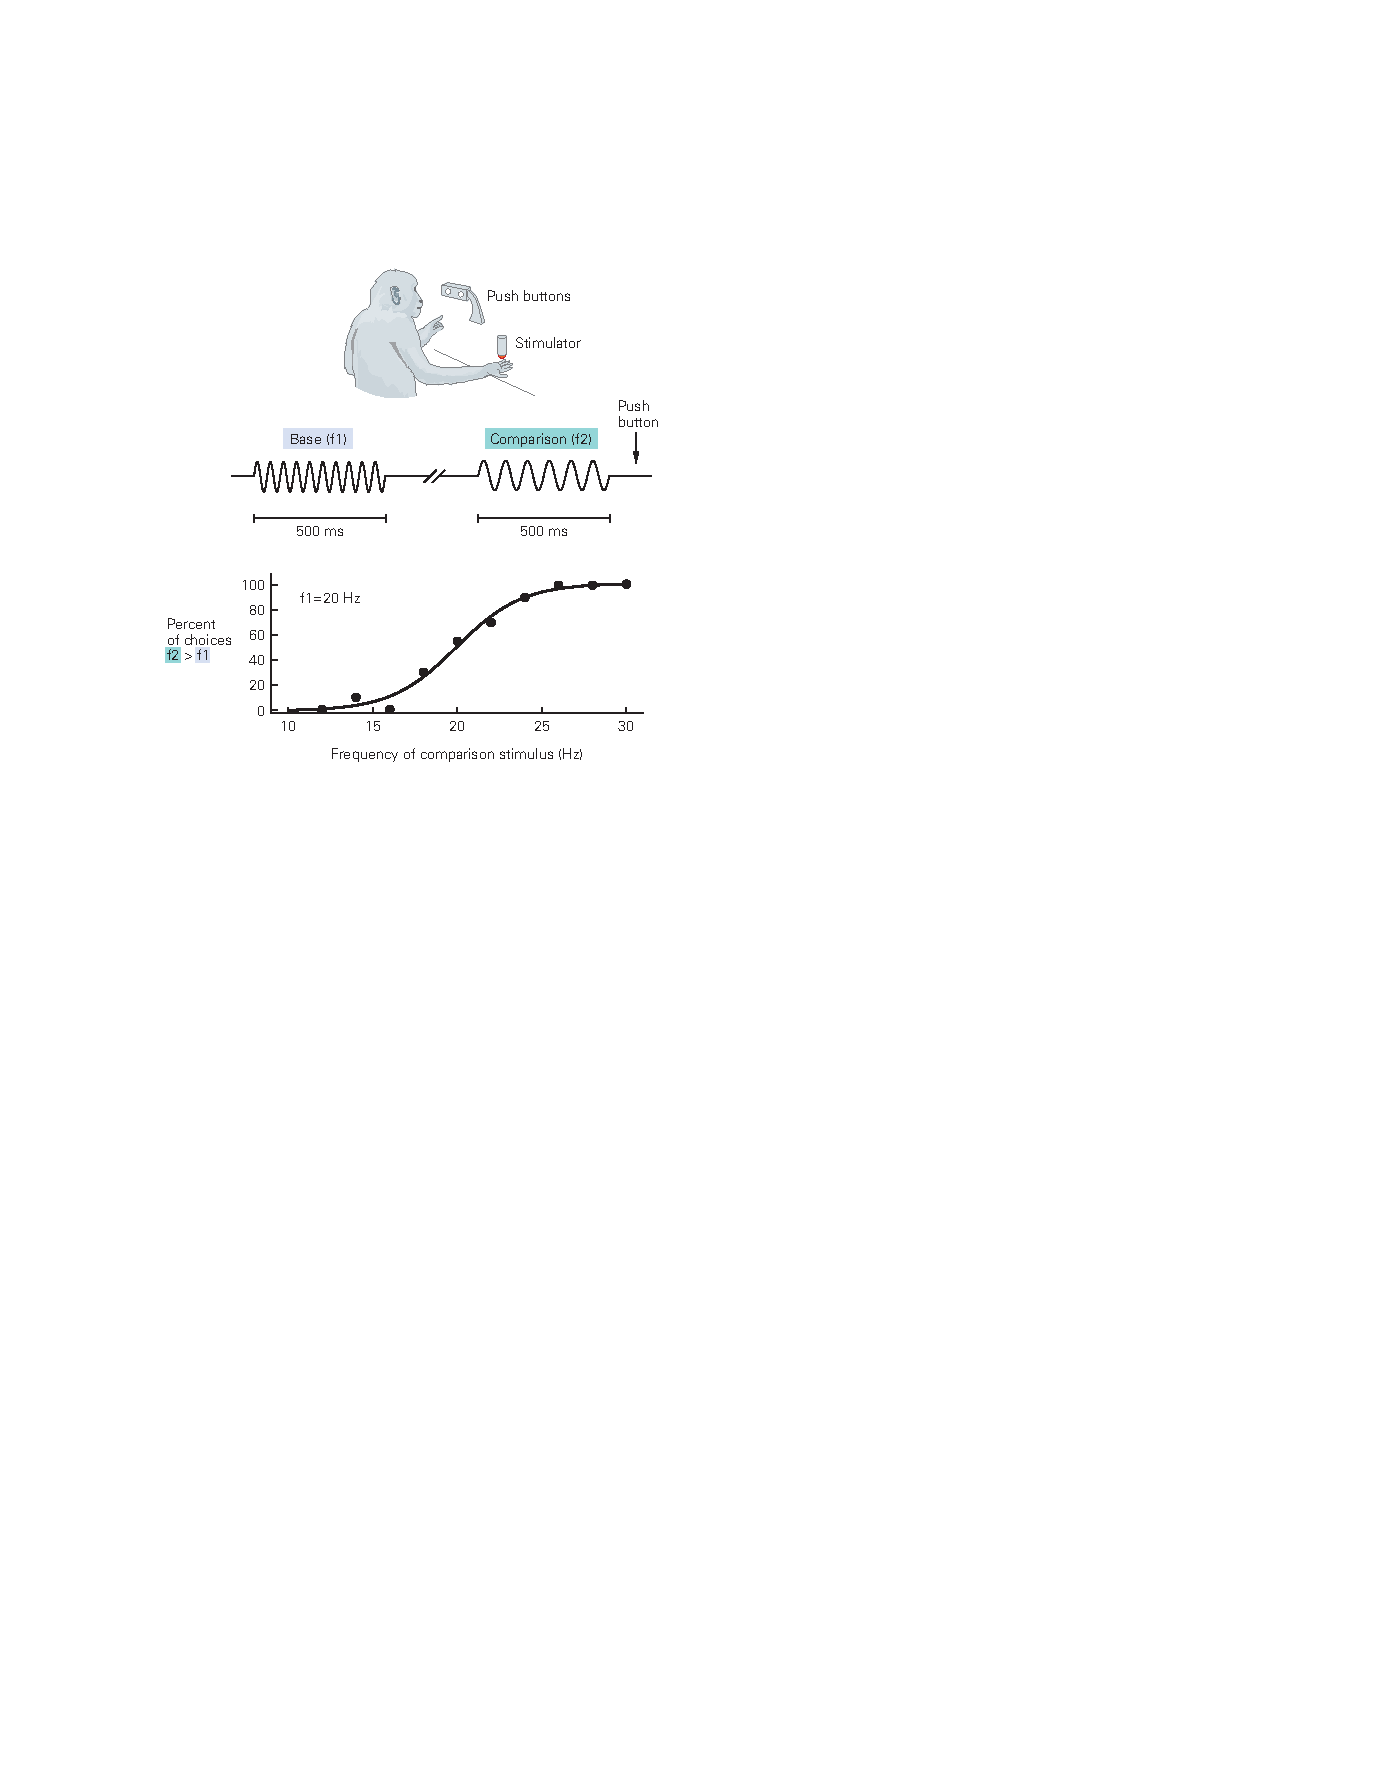
\includegraphics[width=0.7\linewidth]{chap56/fig_56_2}
	\caption{颤振频率的辨别是中枢神经系统研究的第一个知觉决定。
		对右手的手指施加 20 赫兹的振动刺激;
		在几秒钟的延迟时间之后,应用第二次振动刺激。
		猴子通过用另一只手按下左按钮或右按钮来指示第二次振动(f2)的频率是高于还是低于第一次刺激(f1)的频率。
		这些图表明,猴子决定比较刺激大于参考的试验比例取决于差异的大小和符号。
		差异较大时,猴子几乎总是选择正确,但差异较小时,选择往往是错误的\cite{romo2001touch}。}
	\label{fig:56_2}
\end{figure}


我们可以使用我们为检测问题绘制的相同类型的信号和噪声分布在概念上表示该过程(图~\ref{fig:56_1}D)。
此处,“仅噪声”分布表示与 20 赫兹参考相关联的采样量,而红色分布表示与颤动频率大于 20 赫兹的测试刺激相关联的采样量。
\textit{芒卡斯尔}赞成这样的想法,即大脑获得了两个证据样本:一个伴随着 20 赫兹的参考,第二个来自测试。
更高或更低的决定可以通过评估不等式(大于或小于)或等效地通过减去两个样本并根据差异的符号来回答来产生。
这是一个了不起的见解,但神经记录与理论不一致。
\textit{芒卡斯尔}的神经记录解释了猴子检测振动刺激的能力是强度和频率的函数(第~\ref{chap:chap17}~章)(是/否的决定),但他们无法解释两种选择之间的比较机制,无论 f2 更大还是 小于 f1。


缺少两个关键要素。
首先,为了评估 f2 与 f1,大脑需要表示频率。
\textit{芒卡斯尔}在体感皮层和丘脑中发现神经元的放电率与颤动的频率锁相,他们可以测量这种频率锁定的可靠性,但他们没有发现调谐到特定频率小于或大于特定频率的神经元 超过 20 赫兹。
其次,两种表示形式需要同时可用,以便对它们进行比较。
然而,对 f1 的神经反应只持续了与颤振一样长的时间。
\textit{芒卡斯尔}未能观察到神经反应,这些神经反应通过延迟期传达参考频率的表示,直至出现测试刺激。
因此,不可能研究与决策过程相对应的神经操作,这似乎需要在测试分析期间对参考刺激进行一些追踪。


使用更简单的任务设计和不同的感官方式克服了这些障碍。
受到\textit{芒卡斯尔}的启发,\textit{威廉$\cdot$纽瑟姆}训练猴子判断动态随机点场是否倾向于向一个方向或相反方向(例如,向左或向右)移动。
随机点运动刺激的构造使得在一个容易的极端处,所有点都共享相同的运动方向,比如向右。
在另一个容易出现的极端情况下,所有点都向左移动,而在中间,方向可能很难辨别,因为许多点只会产生噪声(图~\ref{fig:56_3}A)。


\begin{figure}[htbp]
	\centering
	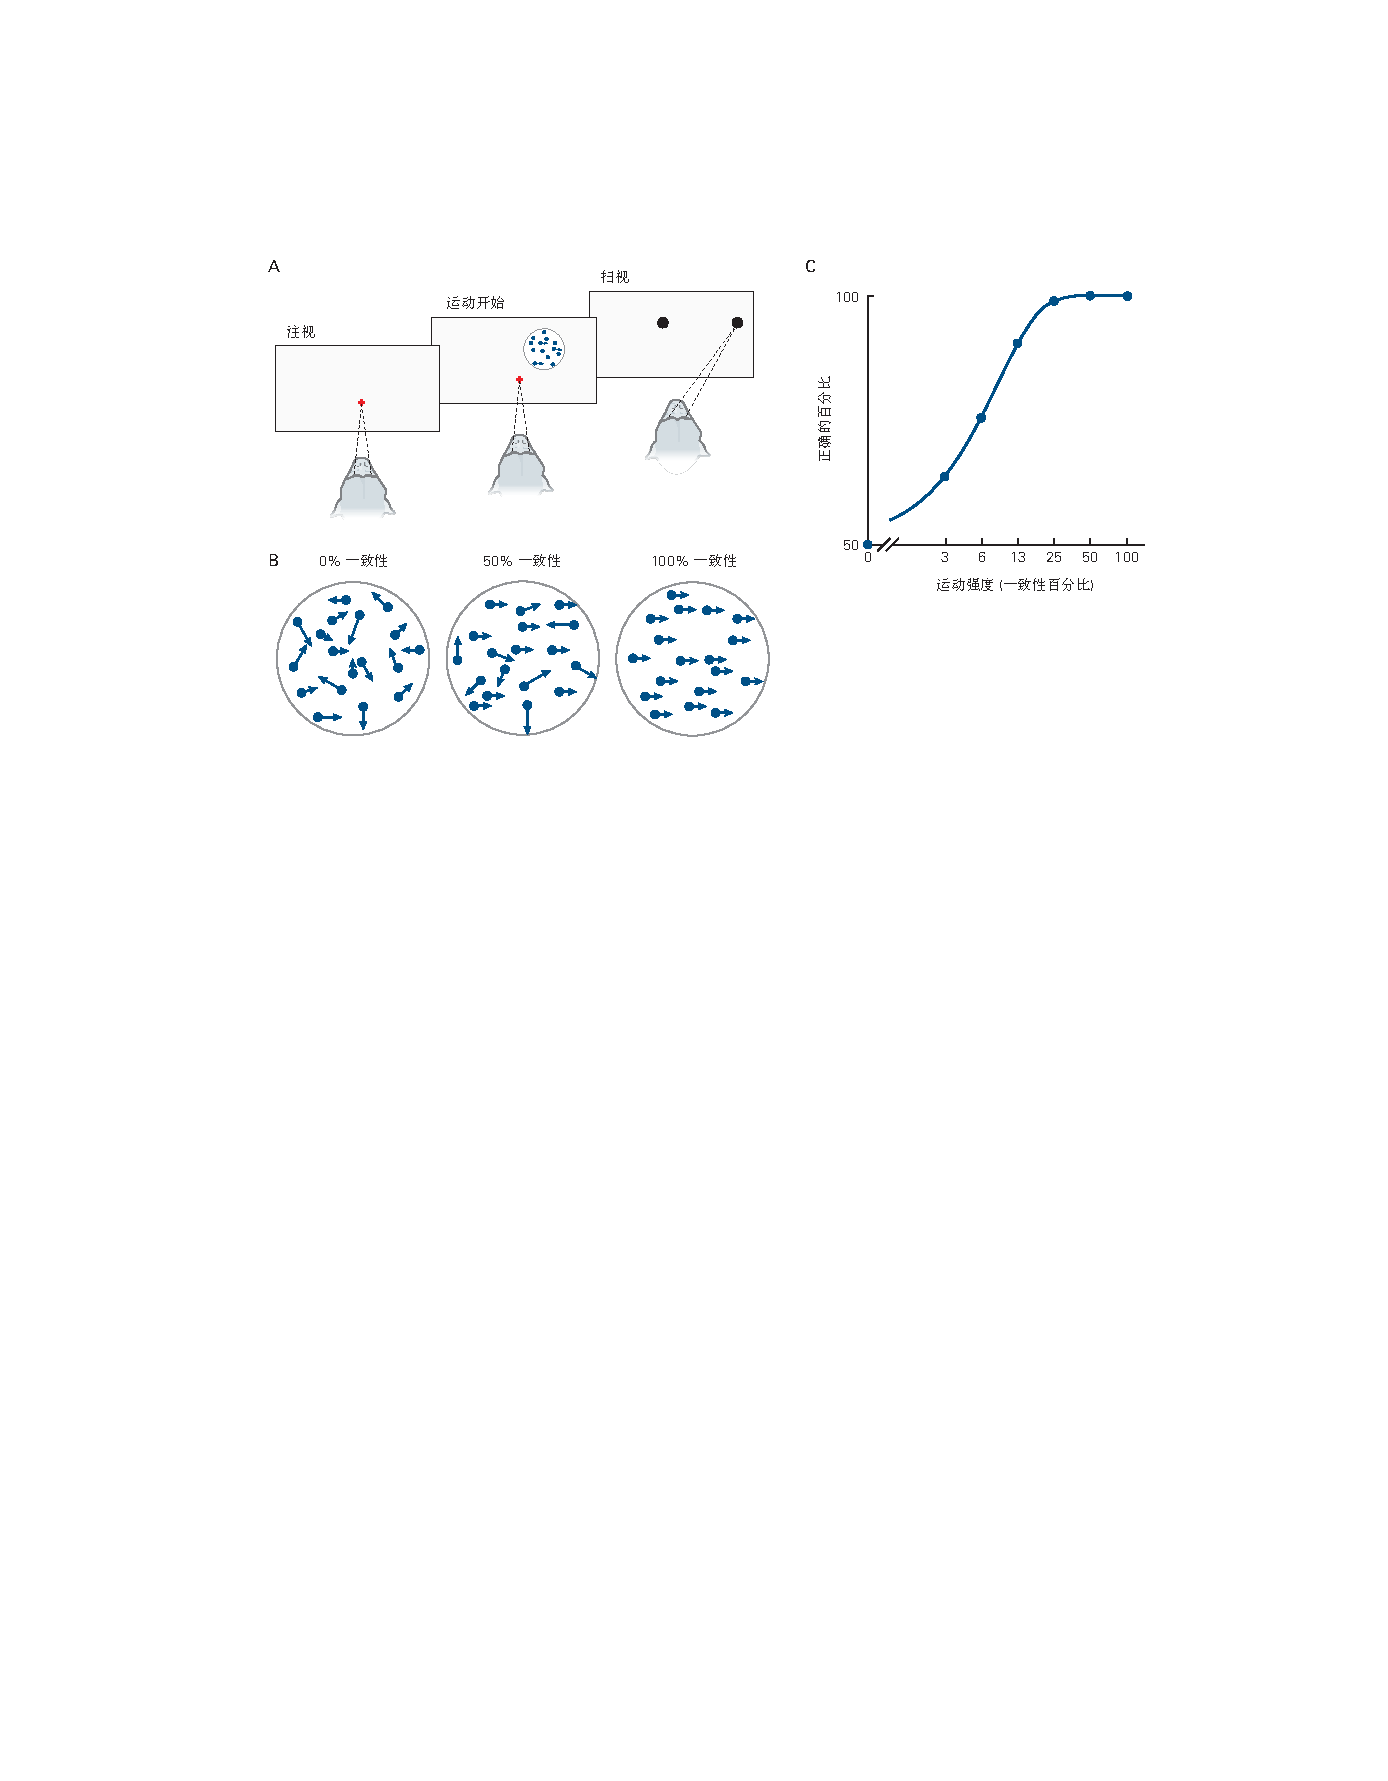
\includegraphics[width=1.0\linewidth]{chap56/fig_56_3}
	\caption{在随机点运动辨别任务中,观察者决定点的净运动是在一个方向还是相反的方向(例如,向右或向左)。
		\textbf{A.} 猴子在观看随机点运动显示时保持注视在十字架上。
		当刺激和注视交叉消失时,猴子通过将目光转移到左侧或右侧选择目标来表示其决定,如果决定正确则获得奖励。
		\textbf{B.} 决定的难度由点运动的连贯性控制。
		每个点在随机位置仅出现几毫秒,然后在 40 毫秒后重新出现,要么出现在新的随机位置,要么出现在与所选速度和方向一致的位移处。
		在时间 $t_1$ 出现的点在时间 $t_2$ 沿相同方向发生位移的概率确定了运动强度(一致性百分比)\cite{britten1992analysis}。
		\textbf{C.} 当运动更强时,决策更可能是正确的。}
	\label{fig:56_3}
\end{figure}


与通过使比较频率更相似而使决策变得困难的颤振任务不同,两个运动方向在所有难度级别下保持固定和相反。
通过降低随机点的信噪比,这两个方向变得不那么明显了。
每个随机点只会短暂出现,然后在随机位置或位移处重新出现以支持一致的方向和速度。
后者(位移)的概率决定了运动强度,通常以 0 到 100 的等级表示,称为百分比相干性。
在最困难的极端情况下,即 0\% 连贯性,所有点都绘制在每个连续帧中的随机位置,呈现出没有主导方向的舞动雪花的外观。
在中等难度下,飞舞的雪花会让人产生一种微弱的感觉,即风可能会将它们稍微向右或向左吹。
任何一个点都不太可能被移动多次,因此没有可追踪的特征。


这个简单的刺激最初是由\textit{安东尼$\cdot$莫夫松}开发的,目的是促进一种决策策略,该策略将受益于在其空间范围内整合视觉信息并作为时间的函数。
此外,它还满足了另一个迫切需要:相同的神经元应该为所有难度级别的决策提供信息。
对于左右决策,视觉皮层中的方向选择性神经元(例如,对向左运动敏感)会发出与所有难度级别的决策相关的信号。
如果难度是由两个方向之间的角度差异控制的,情况就不会是这样。
与振动颤动任务相比,此任务的另一个优点是只有一个刺激呈现。
无需记住参考和测试刺激之间的任何内容。
最后,人类和猴子以几乎相同的水平执行这项任务。
他们完美地回答了强烈运动试验,并在运动强度降低时犯了更多错误(图~\ref{fig:56_3}C)。
这为决策和神经活动的定量协调建立了一个平台。
有没有一种方法可以解释通过测量适当的感觉神经元中的信噪比来做出准确决策的可能性?



\section{皮层感觉区域的神经元为决策提供嘈杂的证据样本}

在高等哺乳动物和灵长类动物中,对运动方向有不同反应的神经元首先出现在\textit{初级视觉皮层}。
它们是\textit{休伯尔}和\textit{威泽尔}(第~\ref{chap:chap22}~章)发现的定向调整的简单和复杂细胞的子集。
这些神经元投射到次级视觉皮层区域\textit{内侧颞叶}区域。


\textit{内侧颞叶}区包含完整的对侧视野图,几乎所有\textit{内侧颞叶}区的神经元都具有方向选择性。
具有相似方向偏好的神经元聚集在一起,因此\textit{内侧颞叶}包含视野中每个点的空间和运动方向图。
它们的感受野大于\textit{初级视觉皮层}神经元的感受野,并且一些显性特性在\textit{初级视觉皮层}中不明显(例如,模式运动;
第~\ref{chap:chap23}~章),但大多数响应就像它们整合来自\textit{初级视觉皮层}的信号,这些信号在更大的范围内具有相同的方向选择性视野的补丁。
在\textit{纽瑟姆}的实验中,随机点运动刺激包含在一个与\textit{内侧颞叶}神经元感受野大小相匹配的圆形孔径中。
因此,有可能测量一个神经元的反应,该神经元完全位于将证据传递给单次试验的决策过程。


似乎有可能,具有与随机点运动刺激对齐的感受野的神经元和对所考虑的一个或另一个方向的发射偏好可能有助于做出决定的证据。
事实上,我们可以通过对\textit{内侧颞叶}神经反应应用相同的信噪比考虑来开始了解猴子对运动的感知。
我们考虑两种类型的方向选择性神经元(图~\ref{fig:56_4})。
一种类型对向右运动的反应比对向左运动的反应更好,并且当向右运动更强时,它会产生更高的发射率。
它还对 0\% 相干刺激的基线以上做出响应,因为随机噪声包含所有运动方向,包括向左和向右,并且当向左运动更强时,它产生较低的发射率(与 0\% 相干相比)(图~\ref{fig:56_4}B)。
另一种类型的神经元对向左运动反应良好。
它表现出与右偏好类型相同的模式,只是方向偏好相反。
神经元还可能分别代表右偏好神经元和左偏好神经元对相同的弱右向刺激的可能放电率。


\begin{figure}[htbp]
	\centering
	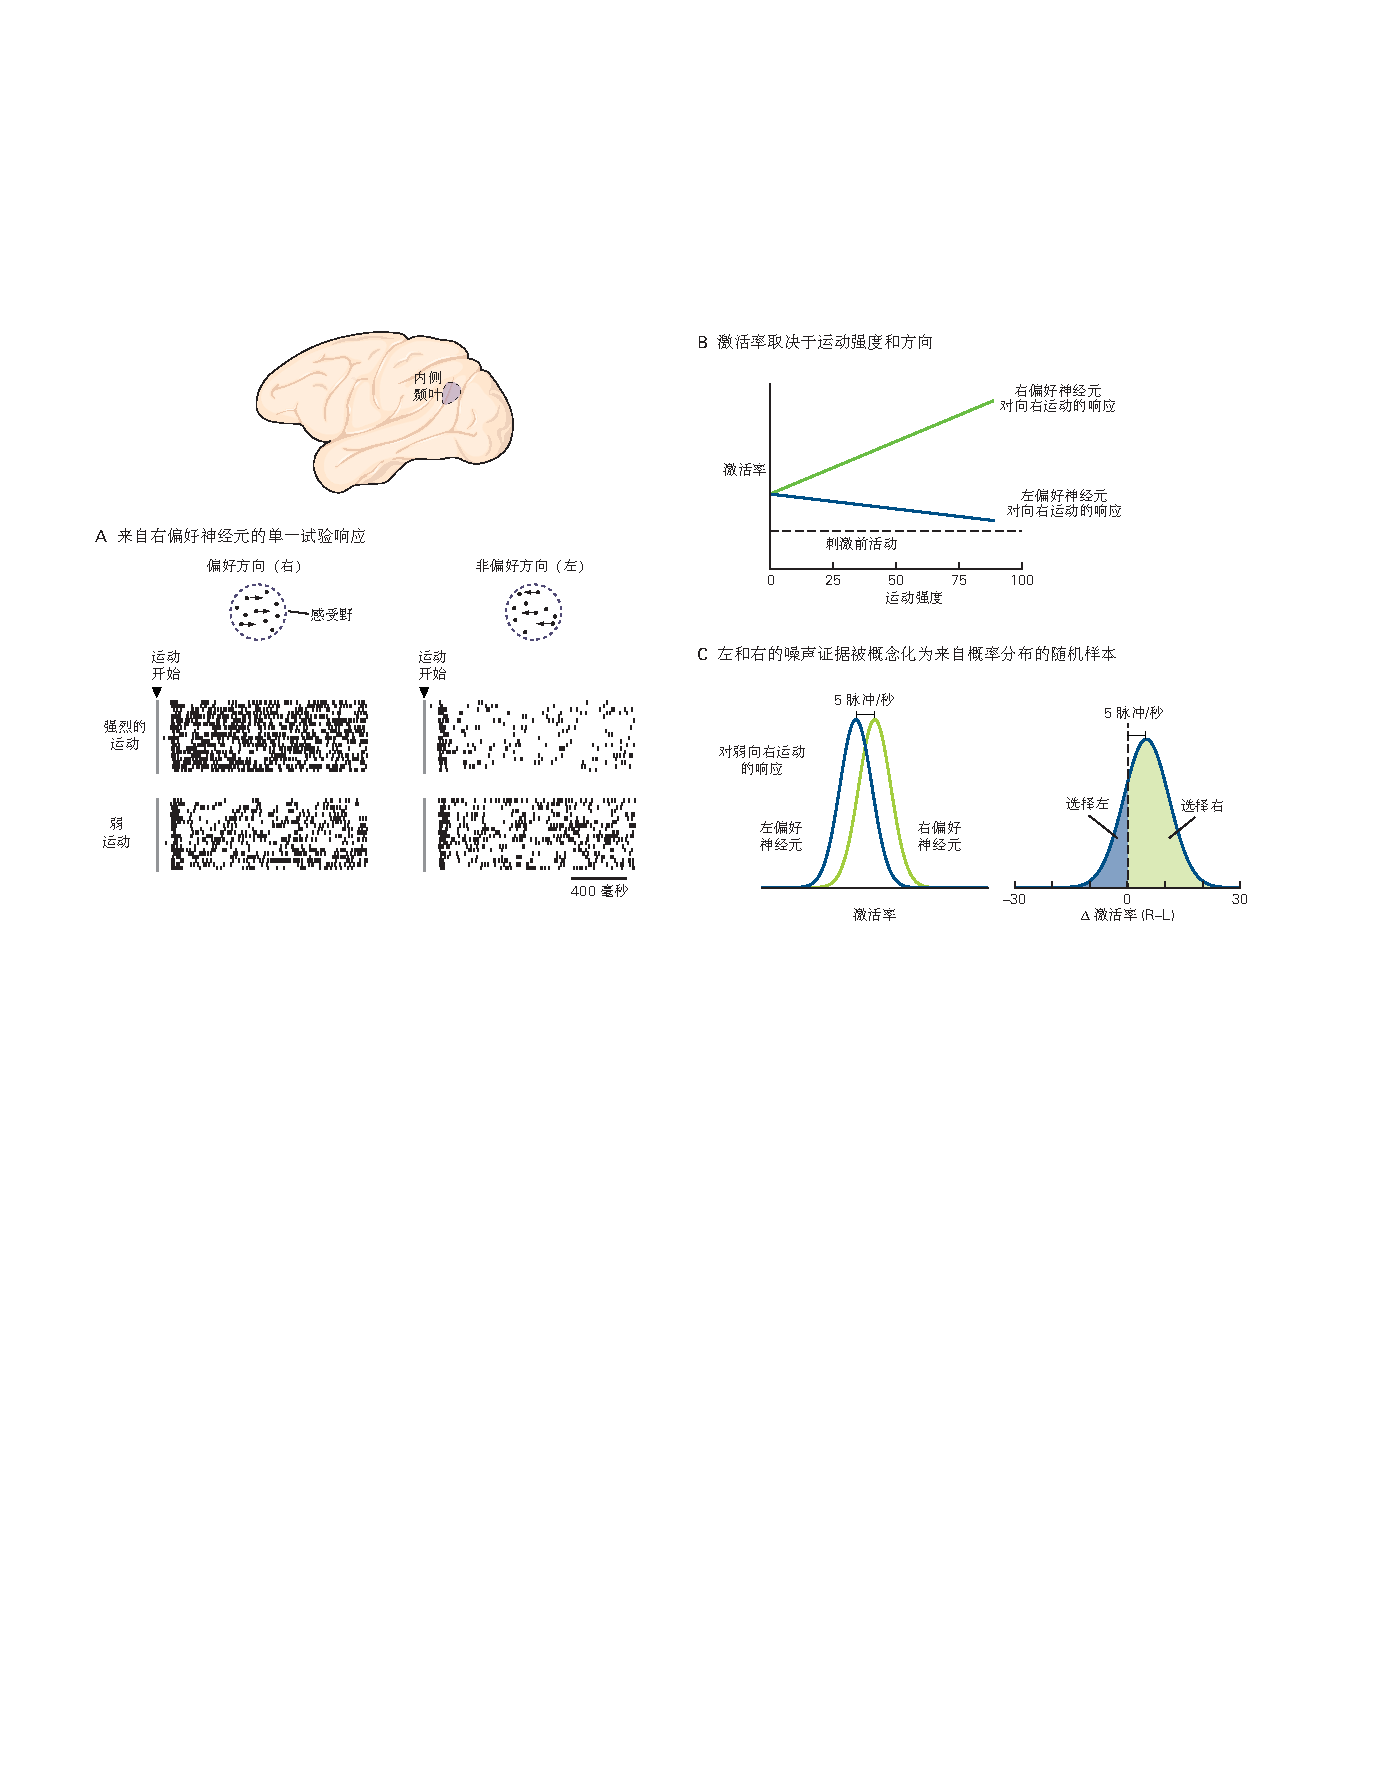
\includegraphics[width=1.0\linewidth]{chap56/fig_56_4}
	\caption{区域\textit{内侧颞叶}中的神经元提供了关于运动方向的噪声证据。
		\textbf{A.} 辨别任务中偏右神经元的反应。 随机点电影在神经元的感受野中。
		2 × 2 面板显示的左列中的面板显示神经元对其首选方向运动的响应,右列中的面板显示其对非首选方向的响应。
		顶行的面板显示神经元对强相干运动的反应,底部面板显示神经元对弱相干运动的反应。
		在每个面板中,每个动作电位(尖峰)的时间由一个小的垂直刻度线表示。
		面板中的每一行尖峰显示神经元在一次试验中对运动刺激的反应\cite{mazurek2003role}。
		\textbf{B.} 平均发射率随运动强度而变化。
		即使响应 0\% 的相干性刺激,神经元也会将其放电率提高到基线以上,因为动态随机点包含所有运动方向,包括神经元的首选方向。
		然后发射率随着更强的向右运动而增加。
		相对于对 0\% 相干性的响应,它随着更强的向左运动而减小。
		这个偏右神经元对向左运动的反应被一个偏左神经元对向右运动的反应所反映。
		\textbf{C.} 从左偏好和右偏好神经元到弱向右运动的放电率的概率分布。
		偏好右侧的神经元往往反应更多,但分布的重叠表明,在任何给定试验中,偏好左侧的神经元可能比偏好右侧的神经元反应更多。
		这些相同的考虑适用于来自右偏好和左偏好神经元群的汇集信号。
		右侧的图显示了在许多试验中响应相同刺激而测得的左偏好神经元和右偏好神经元的放电率之间差异的分布。
		如果差异为正,则决定选择右侧,如果差异为负,则选择左侧。
		这条规则将导致在 80\% 的试验中做出正确的右向选择。}
	\label{fig:56_4}
\end{figure}


因为两类神经元的反应同时可用,我们能够将证据描述为左偏好神经元和右偏好神经元的放电率之间的差异。
(大脑实际上依赖于许多左偏好神经元和许多右偏好神经元的平均值之间的差异。)
我们将这样的数量称为决策变量,因为可以通过对这种差异应用标准来做出决策。
在这里,标准将为零。
因此,如果决策变量为正,则回答正确;
如果是否定的,请向左回答。


请注意,当刺激完全随机(0\% 相干性)时,没有正确答案。
猴子在随机一半的试验中由实验者随机奖励,猴子以大致相等的概率回答左右。
这不是因为猴子在猜测,而是因为随机点运动刺激的波动以及左右偏好神经元的嘈杂放电率导致用于做出决定的证据的可变性。
这是有道理的,因为偏右和偏左的神经元对此类刺激的反应相同。
在一些试验中,偏右的神经元比偏左的神经元反应更多,大脑将此解释为向右运动的证据。
在其他试验中,偏左的神经元反应更多,猴子选择左。


神经科学家已经能够使用由少量神经元组成的网络来模拟动物选择的准确性与运动强度之间的关系,称为心理测量函数。
这些模型的成功支持了这样一种观点,即皮层神经元的信号和噪声特性可以解释知觉决策的准确性,正如蒙卡斯尔所希望的那样。
这一成就之所以成为可能,是因为巧妙的实验设计允许同一个神经元参与各种困难的决策。
但这些神经元真的用来做决定了吗?
他们真的提供了猴子用来做出决定的嘈杂证据吗?


我们现在知道他们这样做了。
由于区域\textit{内侧颞叶}中方向选择性神经元的柱状组织,可以通过微电极施加小电流来激发一组共享相同感受野特性的神经元。
\textit{纽瑟姆}及其同事将电极置于神经元簇的中间,这些神经元的感受野与随机点运动刺激完全一致。
他推断,在弱刺激电流下,大多数受刺激的神经元可能共享相同的感受野和相同的方向偏好。
\textit{纽瑟姆}让猴子在这个方向和相反方向之间做出选择。
例如,如果这些神经元喜欢向右运动,那么弱电流会导致猴子更频繁地决定向右运动(图~\ref{fig:56_5})。


\begin{figure}[htbp]
	\centering
	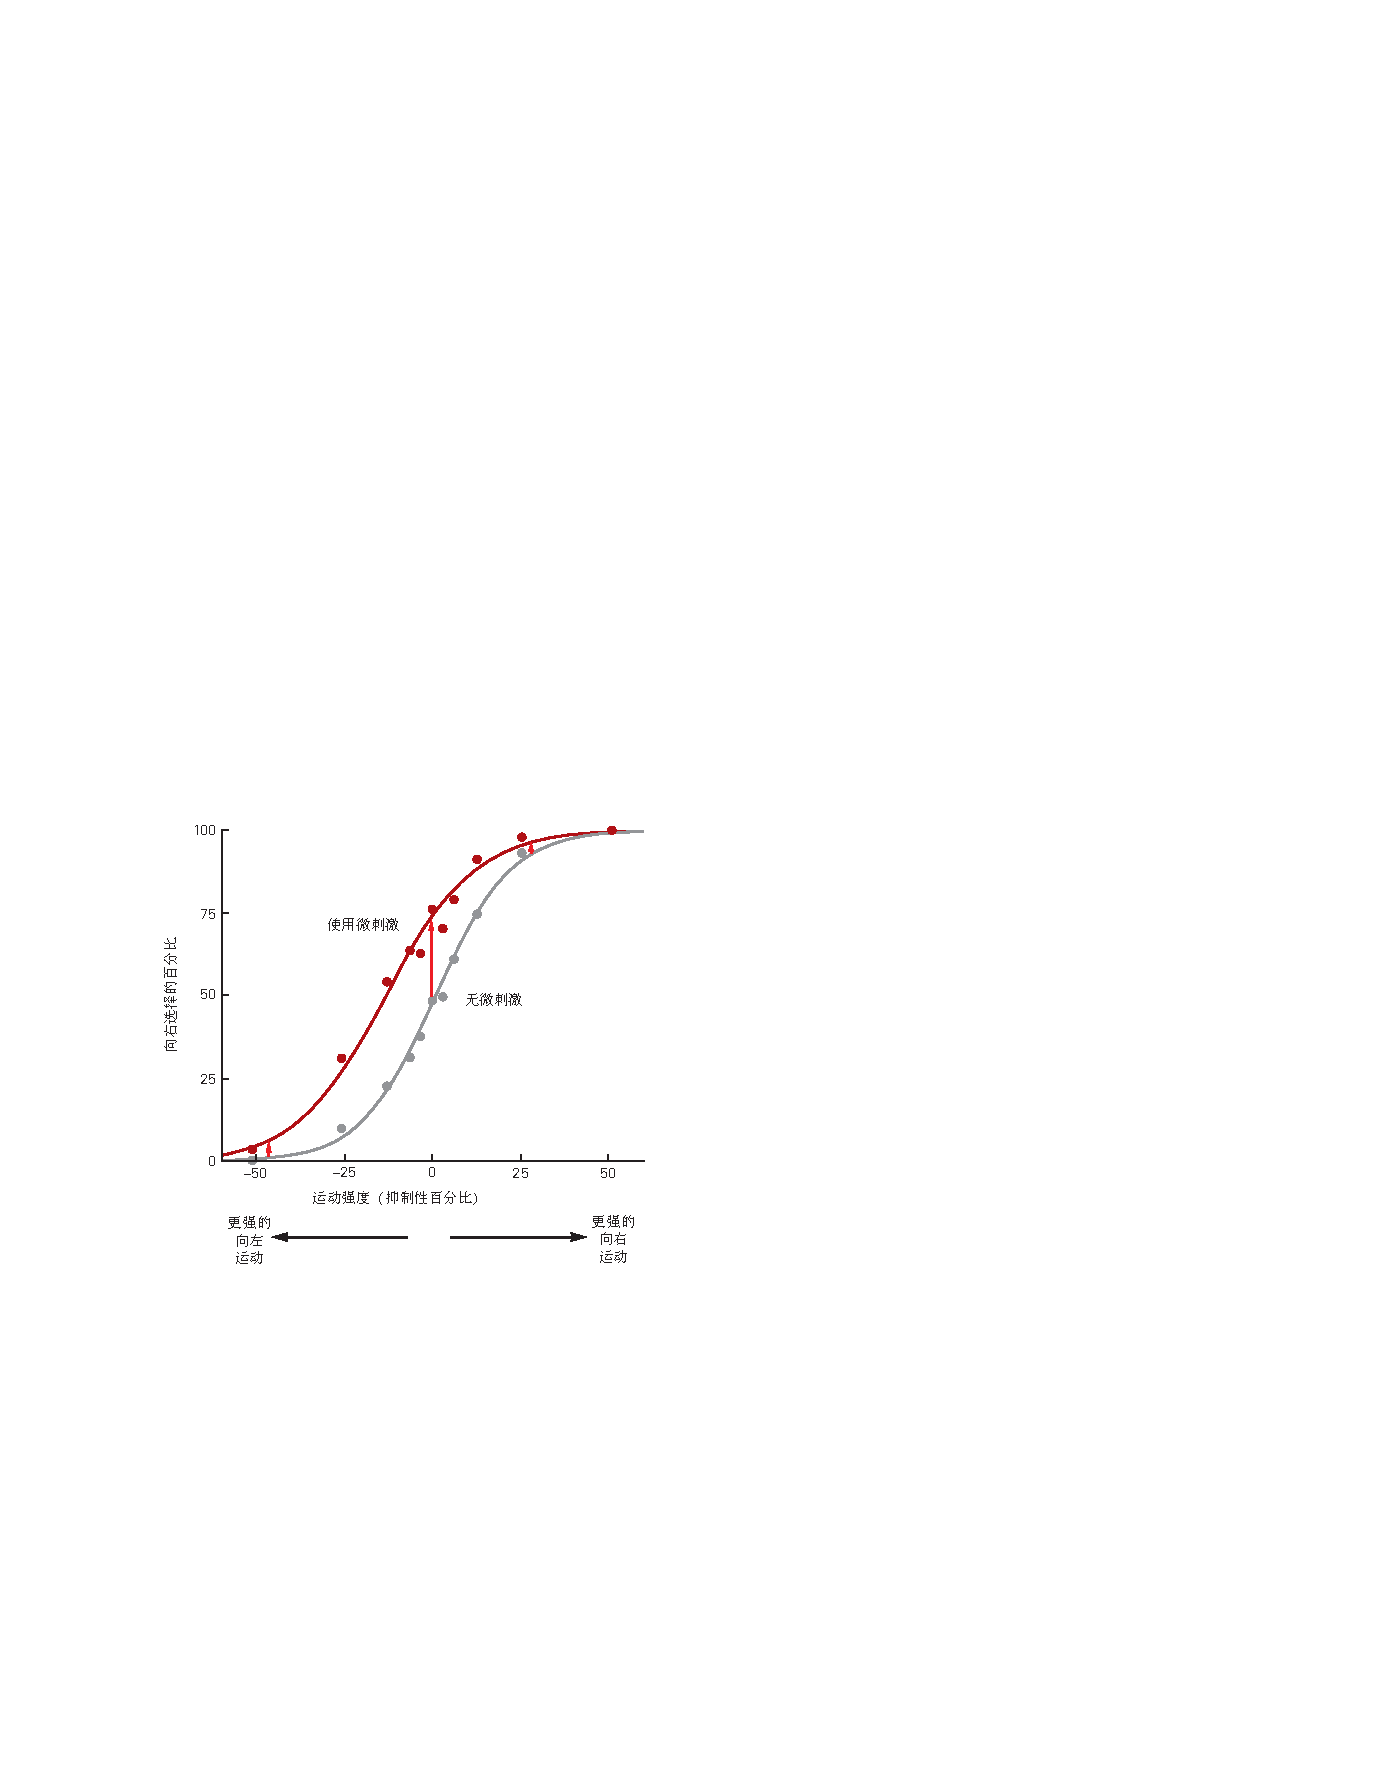
\includegraphics[width=0.66\linewidth]{chap56/fig_56_5}
	\caption{优先响应向右运动的神经元的人工激活导致猴子决定该运动是向右的。
		在实验中,一个电极被放置在\textit{内侧颞叶}区域的神经元补丁的中间,这些神经元喜欢相同的运动方向,比如向右。
		随机点运动显示在这些神经元的感受野中。
		在随机点电影的演示过程中,有一半的试验使用弱交流电。
		电流量可激活电极尖端 50 至 100 微米范围内的约 200 至 400 个神经元。
		在微刺激试验中,猴子更有可能选择模拟神经元的偏好方向。
		当决策更加困难时(中间的红色箭头),效果最为明显\cite{ditterich2003microstimulation}。}
	\label{fig:56_5}
\end{figure}


我们现在将这种旨在影响 50 至 100 微米半径范围内的神经元簇的微弱刺激称为微刺激。
值得注意的是,微刺激不会引起视觉运动的幻觉。
它使猴子的决定产生偏差,猴子的决定主要受随机点运动刺激的引导。
当没有显示刺激时,猴子没有反应,当随机点出现在受刺激神经元感受野之外的视野位置时,微刺激不会影响猴子的决定。
当运动强度最弱时,微刺激对选择的影响最大。
受刺激的神经元只是添加了少量向右运动的证据,这实际上是反对向左运动的证据,如下所述。


微刺激实验表明,区域\textit{内侧颞叶}中的方向选择性神经元为知觉决策提供了证据。
然而,受刺激的神经元不一定需要直接影响决策;
他们只需要参与因果链中的神经回路。
此外,\textit{内侧颞叶}中更多的神经元不受电刺激的影响,但仍然以相同的方向选择性方式对相同的随机点补丁做出响应。
它们位于其他列中,其感受野不以刺激为中心而是与其重叠。
如果移动电极来刺激这些神经元,它们也会使猴子更频繁地选择首选方向。
这些发现表明,在任何一个实验中,微刺激只会影响一小部分有助于做出决定的神经元。
大多数人以他们通常的发射率对随机点运动做出反应。
微刺激只会少量改变大脑用来做出决定的总信号。
难怪效果只有在决策困难时才会显现。


这里有一个重要的原则需要学习。
如果\textit{纽瑟姆}只使用更简单的条件,电刺激就会产生无效效果,因此,神经活动和行为之间的因果关系就不会成立。
最近使用关闭神经元的技术建立了相同的效果模式。
沉默会导致对沉默神经元方向的选择偏差,但这也仅在运动困难时的试验中才会明显。
如果没有充分或必要的证据,神经科学家可能会得出结论,\textit{内侧颞叶}中的神经元不会引起知觉决策的变化。
这将是一个错误,尤其是在任何实验中都可能犯的错误,在这些实验中,扰动仅限于参与计算的神经元子集。
这是高级皮层功能研究的规则,而不是例外。
只有在神经信号总量的微小差异可能会产生影响的条件下研究行为才能缓解这种情况,例如在\textit{纽瑟姆}实验中采用的困难(低信噪比)方案中。


总而言之,感知决策源于一个简单的决策规则:将标准应用于视觉皮层中嘈杂的方向选择性神经元提供的嘈杂证据。
我们将嘈杂的证据描述为一个单一的数字:两个相对的方向选择性神经元池的平均放电率的差异。
该说明遗漏了两个要点:建立决策变量的操作必须由直接或间接从\textit{内侧颞叶}区接收信息的神经元执行,而这些操作需要时间。
正如我们将看到的,时间是理解决策的关键,也是将决策与更高认知功能联系起来的因素。



\section{证据积累到阈值解释了速度与准确性的权衡}

如果大脑只接收到运动的简短快照,比如十分之一秒,那么到目前为止考虑的决策规则是合适的。
然而,决策通常需要一些时间,所以当观看时间越长时,决策往往越准确。
事实上,支持 75\% 准确度所需的运动强度(称为感觉阈值)会随着观看时间的延长而降低。
随着时间的增加,决策者可以用较弱的运动强度达到这种精度水平。
换句话说,对弱运动的敏感度随着观看持续时间 $ t $ 的增加而提高。
事实上,灵敏度的提高是时间平方根(t)的函数,它是通过累积或平均获得的信噪比的改进率。
那么建议是,左偏好和右偏好方向选择性神经元的放电率差异为另一个过程提供了瞬时证据,该过程作为时间的函数积累了这种嘈杂的证据,在这种情况下,两个过程为左偏好积累证据。


噪声证据的积累遵循一条路径,该路径包括在由移动点的连贯性和方向确定的恒定偏差之上的正方向和负方向的随机步骤。
这称为有偏随机游动或漂移加扩散过程(图~\ref{fig:56_6})。
因为支持左的证据就是反对右的证据(反之亦然),所以这两个随机游走是反相关的,尽管并不完全如此。
累积随时间演变并继续这样做,直到刺激被关闭或直到其中一个累积达到上限停止边界,这决定了答案,左或右。
即使是 0\% 的相干性(纯噪声)刺激最终也会达到停止界限,但左积累或右积累这样做的可能性是一样的。
当随机点运动偏向一个方向时,相应的积累更有可能决定选择,并且运动越强越如此。
这种嘈杂证据的积累是决策变量的动态版本。
决策规则仍然相似:如果右侧的证据多于左侧,则选择右侧,反之亦然。
停止边界还解释了决策的另一个重要特征:做出决策所需的时间。


\begin{figure}[htbp]
	\centering
	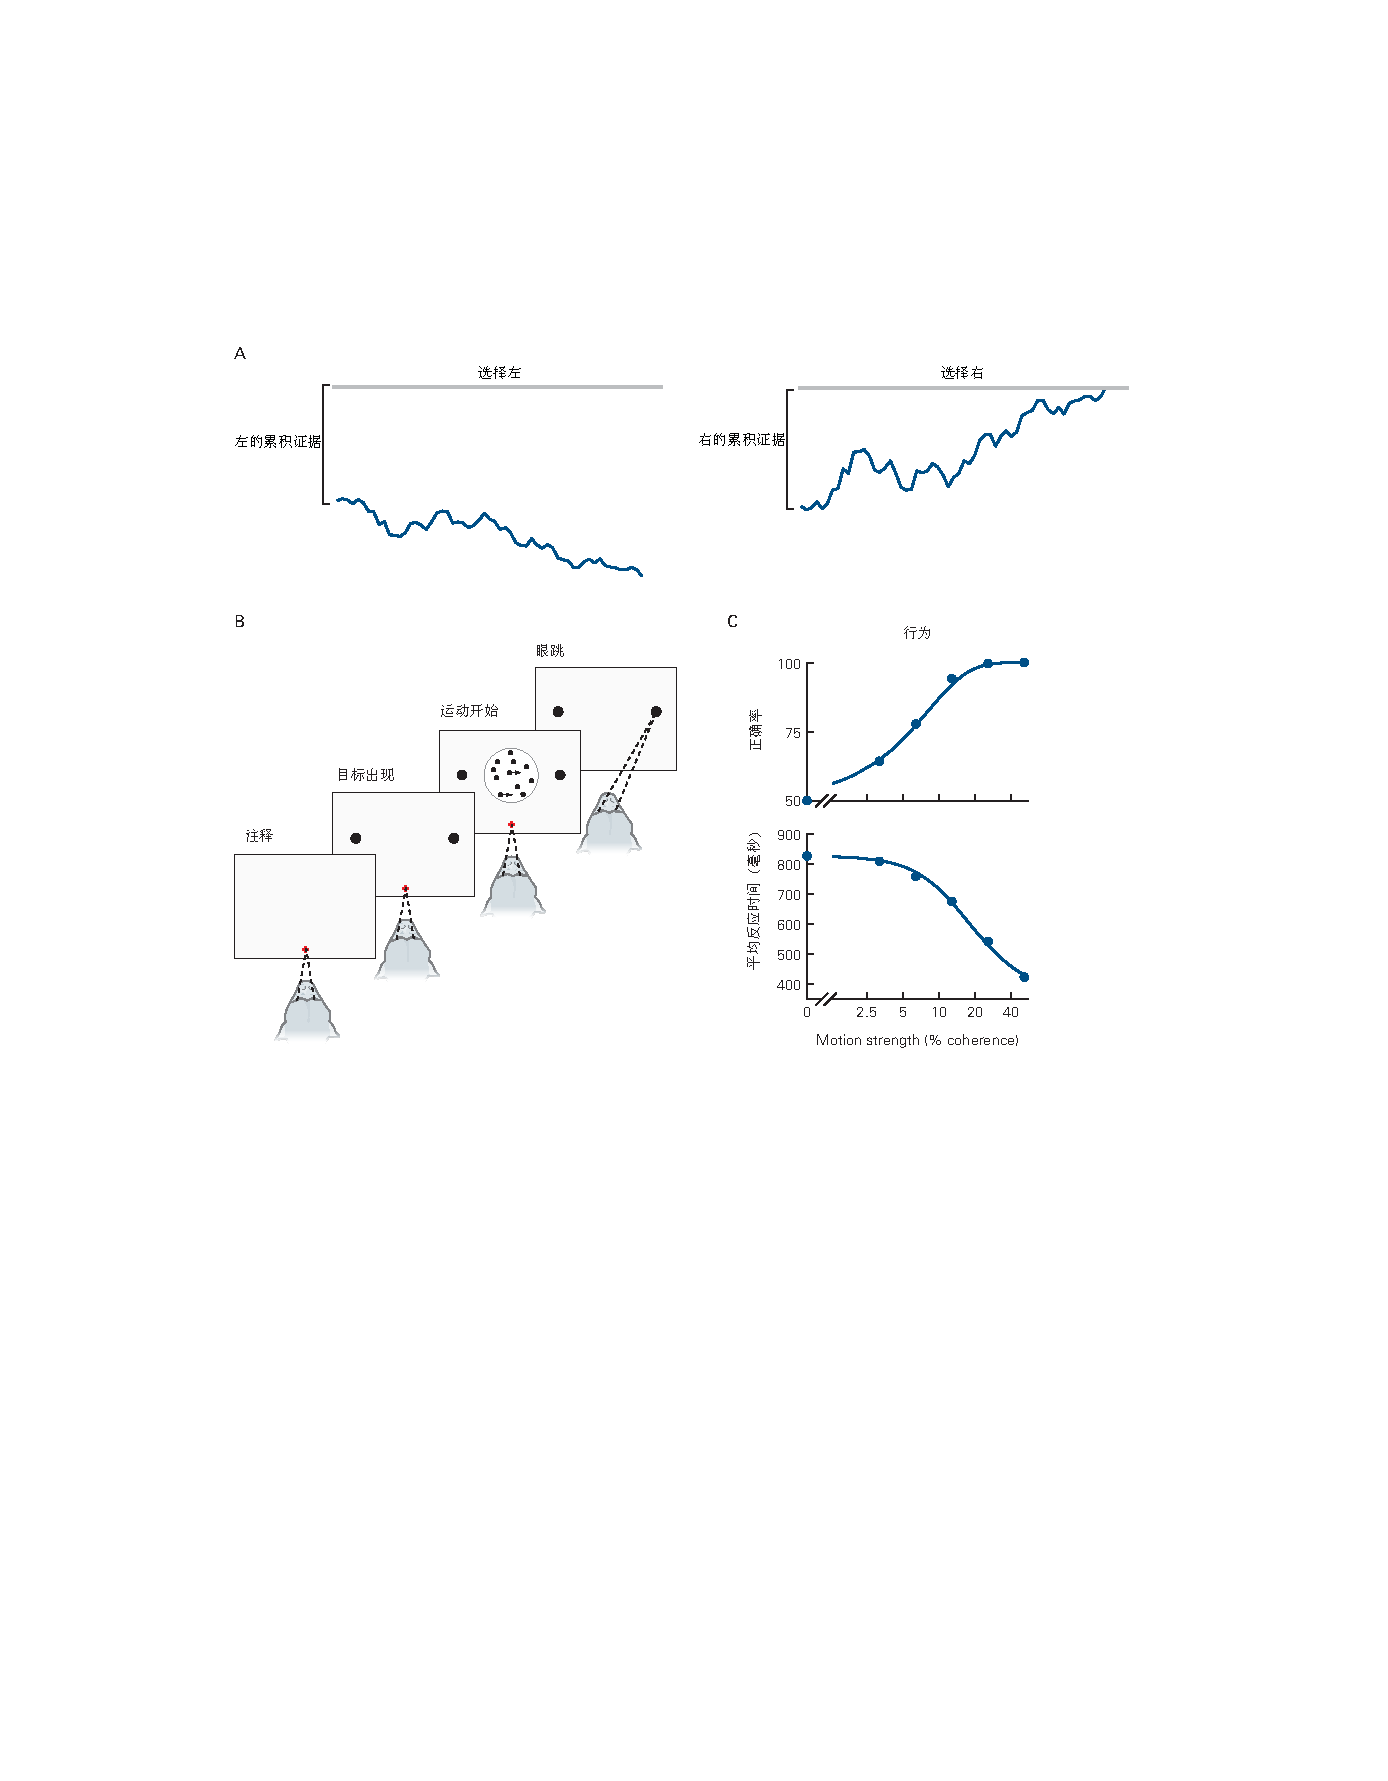
\includegraphics[width=1.0\linewidth]{chap56/fig_56_6}
	\caption{证据积累的过程可以解释决策的速度和准确性。
		\textbf{A.} 决定和做出决定所需的时间都可以通过证据的积累来解释,作为时间的函数,直到有足够的证据终止决定支持一个或另一个选择。
		这幅漫画说明了向右运动的决定,因为“选择正确”的积累是第一个达到停止边界(粗灰线)的。
		因为证据是嘈杂的,所以积累类似于有偏见的随机游走,也称为漂移扩散过程。
		对于左右运动之间的决定,有两个累加。
		左边显示的那个积累了支持左派和反对右派的证据。
		右边显示的那个积累了支持右派和反对左派的证据。
		对于此过程,偏差(或漂移率)是图~\ref{fig:56_4}C 中差异分布(右减左)所描述的证据样本的平均值。
		这个过程是一个随机游走,因为即使运动是向右的,\textit{内侧颞叶}区域中偏左的神经元在任何时刻的反应都可能比偏右的神经元多。
		这两个过程倾向于以反相关的方式发展,因为随机点运动刺激通过视觉皮层为两个积累提供相同的噪声证据样本。
		它们不是完全反相关的,因为偏右和偏左的神经元会引入额外的噪声。
		如果反相关是完美的(例如,如果所有噪声都来自运动刺激),则这两个过程可以用一个累积来表示,该累积在停止上限或停止下限处终止。
		\textbf{B.} 在选择反应时间任务中,决策者在准备好答案时报告决策。
		在这种情况下,猴子通过扫视的方向来表示它的选择。
		\textbf{C.} 图表显示了一个典型的数据集。
		除了正确选择的比例外,\textit{反应时间},即从运动开始到眼球运动反应开始的时间,也取决于运动的强度。
		\textit{反应时间}的总长度是做出决定的时间,由 A 中的过程解释,加上将感觉信息从刺激传递到计算决定的神经元所需的时间,以及将决定转化为运动反应所需的时间\cite{gold2007neural}。 }
	\label{fig:56_6}
\end{figure}


因此,这个简单的想法解释了观察到的决策速度和准确性之间的权衡。
它指定了每个运动强度导致正确选择的概率与平均花费的响应时间(称为反应时间)之间的确切关系(图~\ref{fig:56_6}C)。
如果停止边界接近累积的起点,则决策将基于非常少的证据:快速但容易出错。
如果停止边界离起点更远,则需要更多积累的证据才能停止:更慢但更有可能是正确的。
如果信息流在达到任何一个边界之前就被切断,决策者可能会觉得她还没有得出答案,但仍然可以根据更接近其停止边界的积累来回答。
这种称为有限证据积累的机制解释了任务难度对选择准确性的影响以及对各种感知任务的相关反应时间。
它解释了决策者对决策的信心程度,以及为什么这种信心取决于证据的数量和审议时间。
它还解释了上面提到的当实验者通过 $ t $ 控制观看持续时间时准确性的提高率,并且解释了为什么这种改进随着观看持续时间的延长而饱和。
当累积的证据达到停止界限时,大脑停止获取额外的证据。



\section{顶叶和前额叶联合皮层中的神经元代表一个决策变量}

大脑多个部分的神经元,包括顶叶和\textit{前额皮层},改变它们的放电率以表示证据的积累(在来自\textit{内侧颞叶}区的视觉运动的情况下)与方向决定有关。
代表积累的神经元在两个重要方面不同于感觉神经元。
首先,在感官刺激来来去去后,他们可以继续反应几秒钟。
此外,它们似乎能够将发射率保持在一个水平,然后在新信息到达时增加或降低该水平。
这正是人们希望在代表证据积累的神经元中看到的特征类型。
其次,此类神经元往往与控制行为反应的回路相关联,猴子已经学会用这种回路来传达其决定。
这些神经元最初是因为它们在没有感觉刺激或持续动作的情况下保持持续活动的能力而被识别出来的。
因此,他们被认为在工作(短期)记忆、计划行动或保持对视野中某个位置的注意力方面发挥作用(图~\ref{fig:56_7})。


\begin{figure}[htbp]
	\centering
	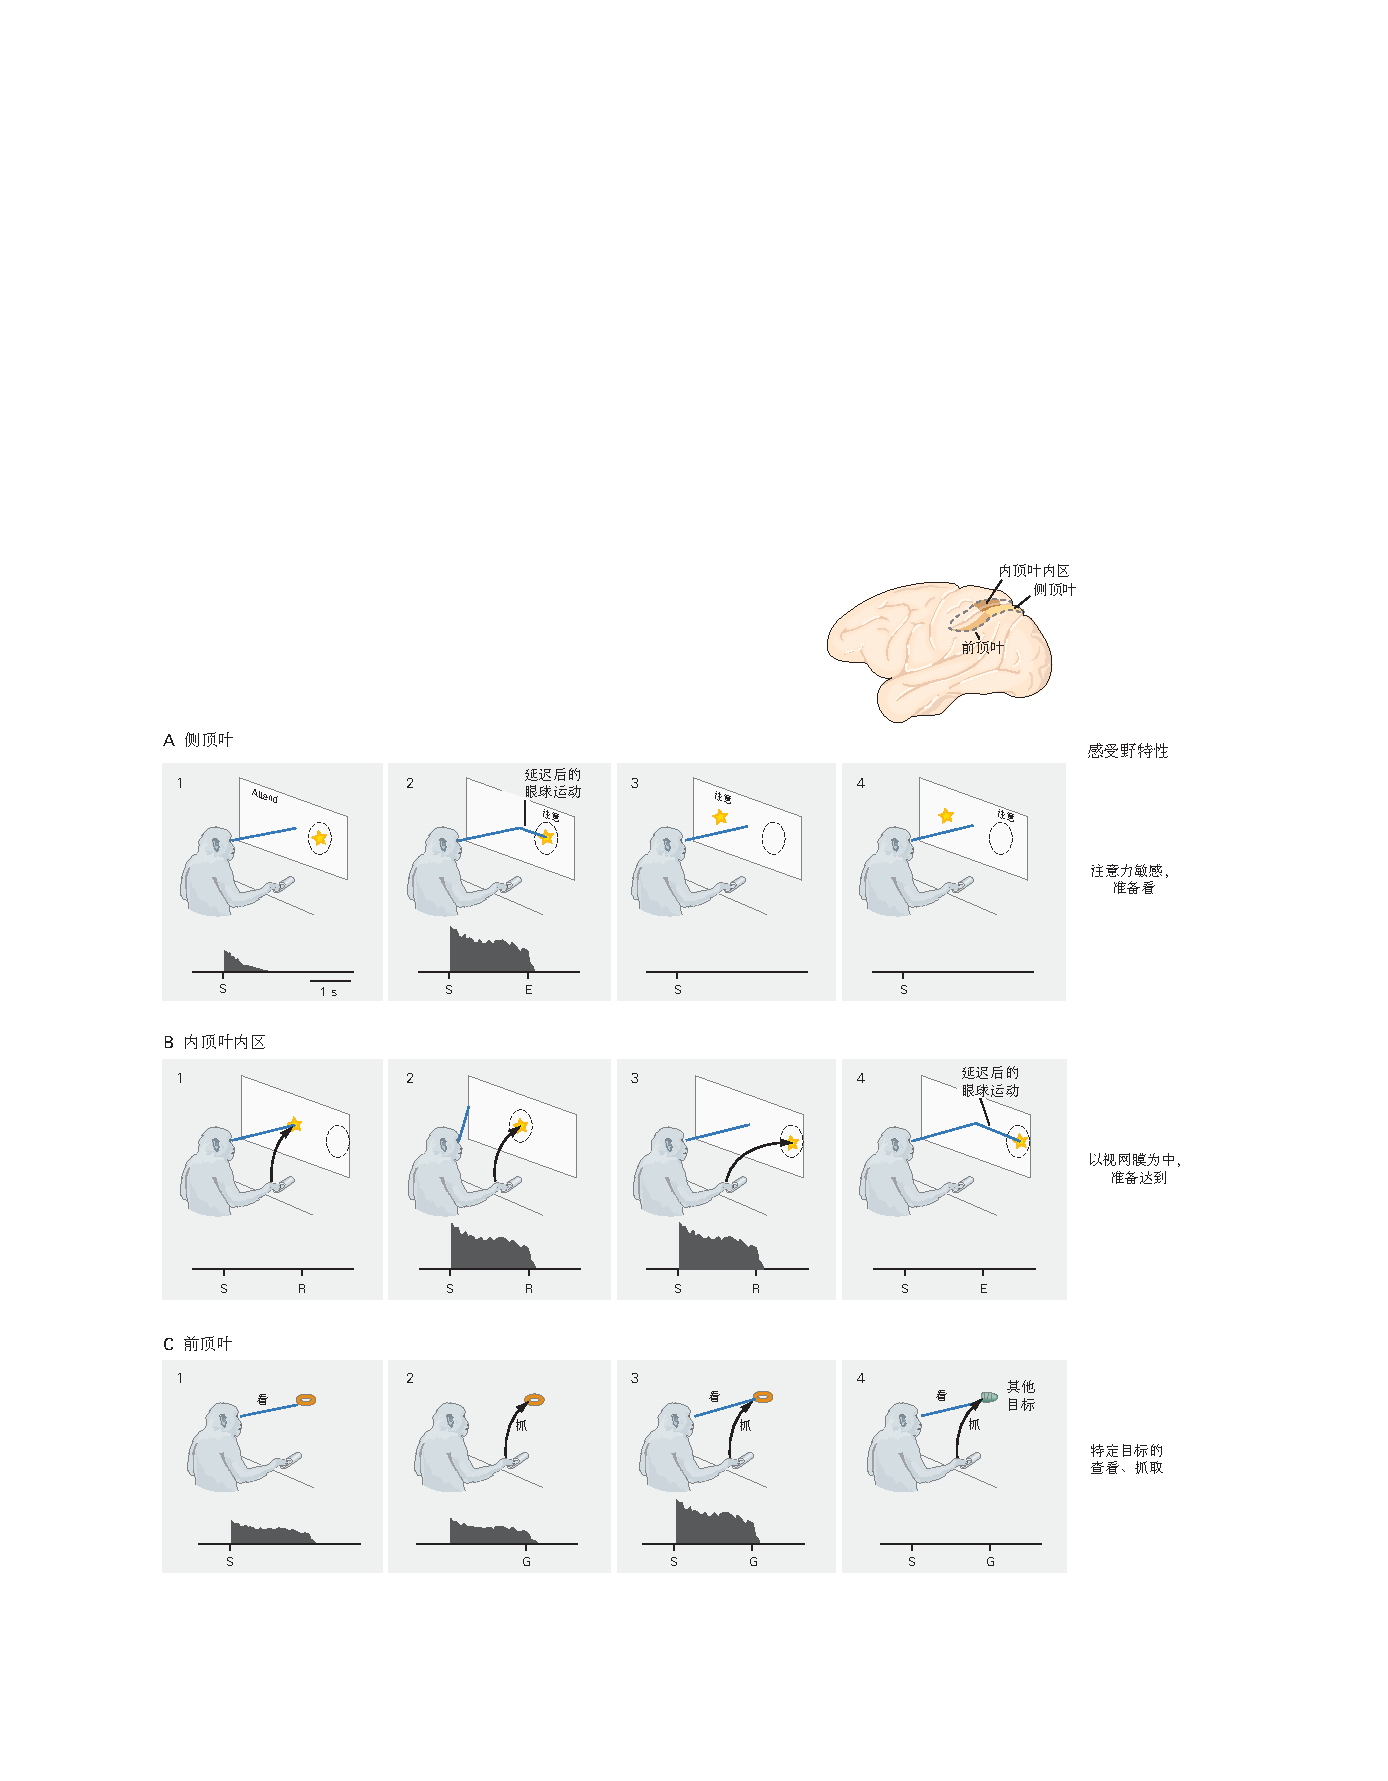
\includegraphics[width=1.0\linewidth]{chap56/fig_56_7}
	\caption{持续的神经活动可以维持工作记忆、注意力和行动计划。
		要求猴子观看场景并通过移动\textit{眼睛}或\textit{伸手}或用手\textit{抓住}来响应\textit{视觉刺激}。
		每个直方图表示一个代表性神经元的放电率作为视觉刺激呈现后时间的函数。
		虚线圆圈显示响应字段。
		这个术语比接受域和运动域更可取,因为这些神经元既不是纯粹的感觉神经元也不是纯粹的运动神经元。
		蓝线显示要求猴子在屏幕上最初注视的位置。
		\textbf{A.} 当猴子准备对物体进行眼球运动或当猴子将注意力转移到物体的位置时,\textit{侧顶叶}中的神经元会放电。
		大多数\textit{侧顶叶}神经元对形状和颜色等目标特征没有选择性。
		当物体出现在神经元的反应场中时,该神经元会激活,该反应场位于猴子正在看的地方右侧的圆圈区域(1)。
		如果在猴子的注意力被引导到这个位置时呈现目标,或者如果猴子被要求计划眼球移动到该位置(2),则神经元的放电会增强。
		在刺激被移除后,激活可以持续几秒钟(2),从而提供了一种潜在的机制来维持对其位置的短期或工作记忆。
		如果目标出现在神经元响应区域之外(例如,左侧)(3),即使要求猴子注意神经元响应区域(4)的位置,神经元也不会放电。
		一个目标必须出现在那里,即使只是短暂的(2)。
		\textbf{B.} 在\textit{内顶叶内区},当猴子准备触及视觉目标时,神经元会放电。
		这个神经元在神经元的反应场中出现目标后不久就开始放电,在这种情况下,猴子正在看的地方右边有一个固定的角度,无论它的目光是在左边缘(2)还是在中心(3)的屏幕,它会在猴子等待到达时继续激活。
		当猴子到达其注视中心的目标时(1)或当猴子计划将其视线转移到反应场中的目标但未到达时(4),神经元不会激活。
		伸展的物理方向不是神经元放电的一个因素:它在 1 和 2 中是相同的,但神经元仅在 2 中放电。
		看着或准备抓住一个物体,并对特定形状的物体有选择性。
		当猴子看到一个戒指(1)或在黑暗中根据记忆伸手去拿它(2)时,这个神经元就会激活。
		当猴子在视觉引导下抓住环时,它会特别强烈地发射(3)。
		它不会在查看或抓取其他物体(4)时触发。}
	\label{fig:56_7}
\end{figure}


其活动代表行动计划的神经元似乎也可能代表决策过程中该计划的形成。
例如,如果一只猴子学会了通过将手移到触摸屏上的目标来回答“向右”,感兴趣的神经元将倾向于与该动作相关联,并且如果猴子计划这样做,它们将减少它们的活动 达到相反的“向左”目标。
这些神经元投射到控制伸手动作的大脑区域。 如果猴子学会了用眼球运动来回答,帮助计划眼球运动到选择目标的神经元就代表了决策变量。
此类神经元已在\textit{侧顶叶}中得到广泛研究。
事实上,这些\textit{侧顶叶}神经元为神经科学家提供了决策过程及时展开的第一视图。


代表进化决策的神经元随着其中一种选择的证据增加而逐渐增加它们的放电率,而当证据支持另一种选择时它们逐渐减少(图~\ref{fig:56_8})。
它们的发射率,绘制为时间的函数,近似于一个斜坡:基线率加上一个常数乘以时间,其中常数与瞬间证据的强度成正比(例如,右侧发射率的平均差异 - 和偏左的\textit{内侧颞叶}神经元)。
这捕获了许多试验的平均发射率,但它遗漏了关键点,即决策变量是信号和噪声的累积。
信号是差值的平均值。 噪声是方差,即均值周围的分布。
累积噪声被图~\ref{fig:56_8}~中的平均值所掩盖,但在多个决策的发射率可变性中很明显。


\begin{figure}[htbp]
	\centering
	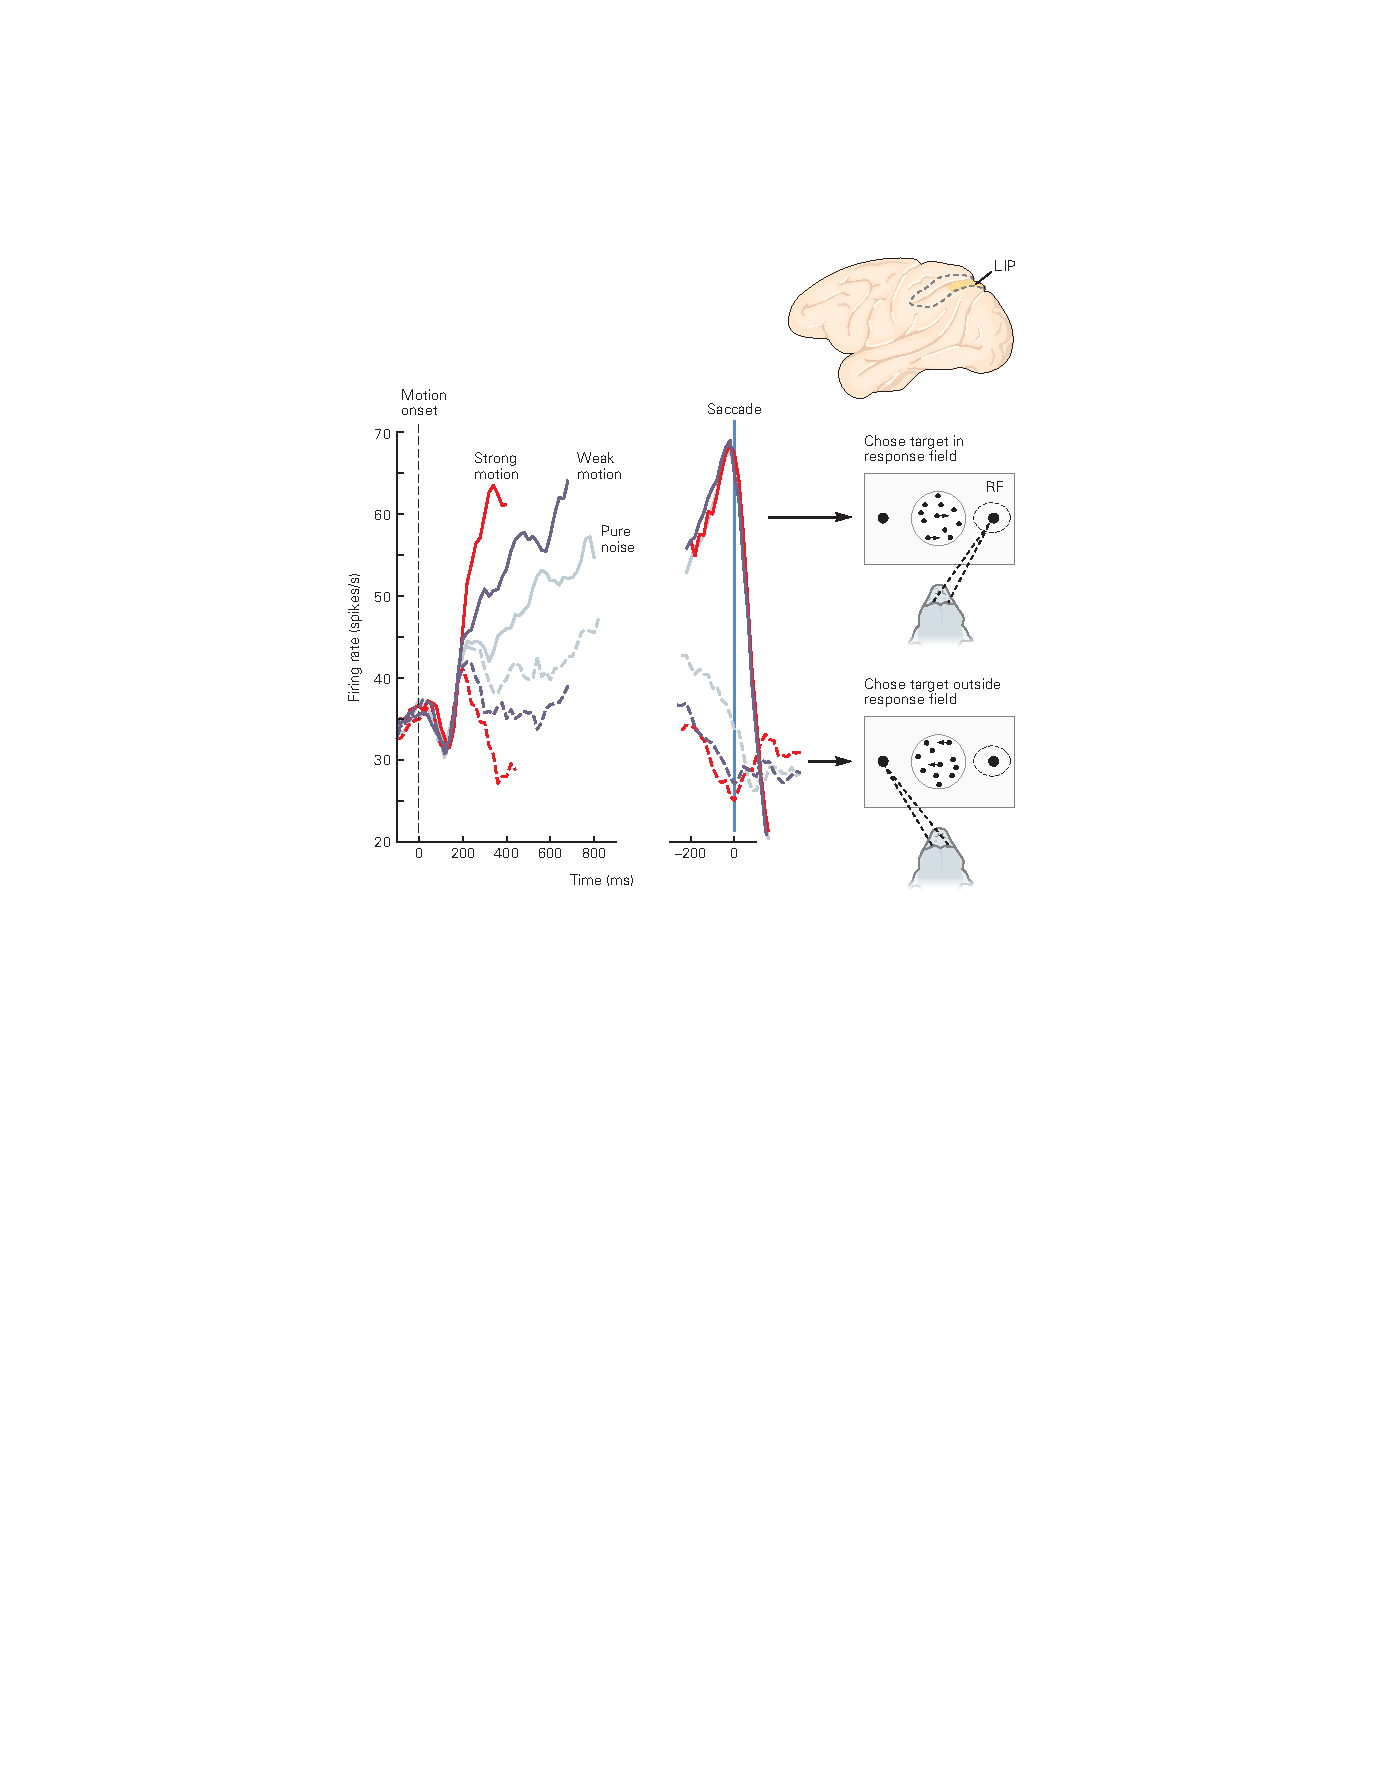
\includegraphics[width=0.86\linewidth]{chap56/fig_56_8}
	\caption{\textit{侧顶叶}中的神经元代表嘈杂证据的积累。
		这些神经记录是在猴子执行动作任务的反应时间版本时获得的。
		这些痕迹是 55 个神经元的平均放电率。
		神经元与图~\ref{fig:56_7}A 中所示的类型相同。
		轨迹显示对三种运动强度的平均响应:强(红色)、弱(紫色)和零(纯噪声,灰色)。
		实线来自猴子在神经元\textit{响应场}(正确选择)中选择目标的试验。
		虚线来自猴子选择神经元反应场之外的目标(左选择)的试验。
		对于非零强度,随机点运动的方向是猴子选择的方向(即,只显示正确的选择)。
		左侧图中的响应与随机点运动的开始对齐,表现出逐渐增强的活动,导致向右选择,以及活动逐渐下降,导致向左选择。
		这种上升和下降的速度反映了运动的强度和方向。
		右边的反应是对相同的点运动,但现在与猴子进行眼球运动(扫视)以指示其选择并揭示其反应时间的时刻对齐。
		就在猴子做出选择之前,反应达到了一个共同水平,这与应用于放电率的阈值确定这些试验的终止的想法一致。
		在向左选择之前,反应没有达到一个共同的水平,因为当一个单独的神经元群在其反应域中具有左选择目标时,这些决定被终止,达到阈值放电率\cite{roitman2002response}。}
	\label{fig:56_8}
\end{figure}


反应从一个共同的水平开始,并随着大脑获得越来越多的信息而演变,直到某些东西停止了这个过程。
停止规则的神经特征在与眼球运动本身一致的反应中很明显。
在只需零点几秒的试验和长达一整秒的试验中,发射率似乎达到了相同的水平。
在眼睛开始移动之前不到十分之一秒就达到了这个水平。
当然,如果发射率快速增加(例如,图~\ref{fig:56_8} 中的红色实线),则达到此水平所需的时间会更短。 这表明当累积证据的表示达到阈值时,大脑会终止决策。
这正是有界积累框架所预测的。
当猴子选择相反的方向时,神经元中似乎没有共同的活动水平来发出向右运动的信号。
取而代之的是,另一群神经元积累了支持左(和反对右)的证据,达到了它们的阈值,并在猴子回答左时终止了决策过程(图~\ref{fig:56_6}A)。
支持正确选择的神经元只是在由左选择神经元确定的时间停止收集证据。
这解释了为什么图~\ref{fig:56_8} 中的向下轨迹在眼球运动期间没有达到常见的活动水平。
目前还不知道阈值操作在大脑的什么地方应用。
计算理论家提出,一个可能的候选者是纹状体,这是一个参与在竞争行为之间进行选择的大脑区域(第~\ref{chap:chap38}~章),但还有许多其他候选结构,包括皮层和脑干的运动区域。


\textit{侧顶叶}区域并不是大脑中唯一代表决策证据积累的部分,\textit{侧顶叶}本身也不限于对随机点运动做出决策。
顶叶和前额叶皮层中的许多神经元表现出持续放电。
事实上,第一个表现出这种活动的大脑区域是在额叶,靠近初级运动皮层,并且在运动皮层本身中发现了一些具有这种特性的神经元。
正如第~\ref{chap:chap52}~章所讨论的,持续性活动被认为代表了空间位置或规则、类别或行动计划的工作记忆。
但是这些神经元也能够代表活动的分级水平,表明具有代表更多信息的能力 模拟量,例如不断变化的决策变量、采取行动的预期价值或感官质量的工作记忆,正如我们接下来要考虑的那样。


在\textit{芒卡斯尔}发表他的颤振辨别研究 20 年后,他的学生\textit{拉努尔福$\cdot$罗莫}通过关注前额叶皮层中的神经元使这一研究重新焕发活力,前额叶皮层具有我们一直在讨论的那种持续活动。
罗莫修改了任务。
猴子仍然面临两个振动刺激,间隔一定时间,并且需要决定第二个刺激的振动频率(f2)是否大于或小于第一个刺激的振动频率(f1)。
然而,不是在所有试验中使用相同的 20 赫兹参考刺激,而是在试验中颤动频率不同。
他发现,在猴子等待第二次刺激的延迟期间,前额叶皮层中的许多神经元以分级和持续的方式对第一次颤振刺激的频率做出反应。
一些神经元的放电率随着 f1 的振动频率而增加,而其他神经元在频率较低时更加活跃。
\textit{芒卡斯尔}在他最初的研究中没有观察到这些持续的神经反应。
有证据表明,决策变量是在腹侧前运动皮层中构建的,神经元对差异 f2 – f1 做出反应。
这很难研究,因为决策变量不会在很长一段时间内演变。 无需获取大量证据样本。
所需要的只是对 f2 的估计和阈值的应用。
颤振任务通过展示持续活动的多种功能来补充运动决策任务。
在运动任务中,持久性支持决策变量的计算:对决策备选方案的累积证据。
在颤振任务中,持续活动代表一种感觉质量(参考刺激的频率)通过延迟期。



\section{感知决策是从证据样本进行推理的模型}

动物和人类做出的大多数决定与微弱或嘈杂的感官刺激无关。
它们与活动、购买、提议和菜单项有关。
他们从个人经验、书籍、朋友和电子表格等来源获得知识和期望。
有些基于内部(主观)估值或偏好。
许多涉及从可靠性可能不同的证据来源进行推理,并且必须权衡成本和收益。
感知决策的神经机制在多大程度上适用于这些其他类型的决策?


想象一下以下场景。
早上离开家时,您意识到下午 4 点到 5 点您将在户外,必须决定是否带伞。
为了使这变得有趣,假设这发生在互联网和准确的卫星天气预报时代之前。
您必须根据昨天“可能下雨”的预报、早上 7:00 天空的晴朗外观、与 1 小时前相比气压的小幅下降以及观察到的十几个行人中的观察结果来做出决定。
你的窗户只有一个,似乎拿着一把雨伞。
让我们进一步假设您有做出此类决策的经验,并且对这些指标的可靠性有一定了解。
最后,携带雨伞的繁琐使得您的决定归结为对是否更有可能下雨的合理评估。


做出此决定的正确方法是考虑每个指标,并询问如果下午下雨或不下雨,它们的可能性有多大。
这些似然是条件概率的学习估计,下午下雨时观察指标的概率,不下雨时观察到相同观察结果的概率。
例如,假设您通过经验了解到下雨的可能性预报意味着下雨的可能性为四分之一。
那么,根据天气预报,下雨或不下雨的条件概率分别为四分之一和四分之三。
这两个概率的比率称为\textit{似然比},在这种情况下为 1 比 3。
如果\textit{似然比}大于 1,则有利于下雨,如果\textit{似然比}小于 1,则有利于不下雨。
四个指标各有一个\textit{似然比}。
如果四个\textit{似然比}的乘积大于 1,那么你应该带伞。


出于稍后会清楚的原因,取\textit{似然比}的对数很有用,称为\textit{对数似然比}。
这为信念提供了一个更自然的尺度,它允许我们用加法代替乘法 [回想一下$\text{log}(xy) = \text{log}(x) + \text{log}(y) $。
为了理解这个比例,假设一个带雨伞的路人无论是否下雨都同样有可能带伞。
两个概率都是 1 比 2。
因此\textit{似然比}为 1,log(1)=0,这对应于这种观察没有提供信息的直觉。
大于 1 的\textit{似然比}取正对数,小于 1 的\textit{似然比}取负对数,与预测降雨的方式一致。


可以训练猴子执行此天气预报任务的一个版本。
在图~\ref{fig:56_9}~所示的实验中,一只猴子必须决定是看红色还是绿色目标,只有其中一个会导致奖励。
在选择红色或绿色之前,向猴子展示了四种形状。
每一个都作为奖励位置的指示器。
这只猴子学会了将预测值与总共 10 种形状相关联,其中一半喜欢红色的奖励,另一半喜欢绿色。
这些形状在预测奖励位置的可靠性方面也有所不同。
猴子学会了理性地依赖这些形状,通过结合每种形状的证据并通过给予信息量更大的形状更多的选择权来做出决定。


\begin{figure}[htbp]
	\centering
	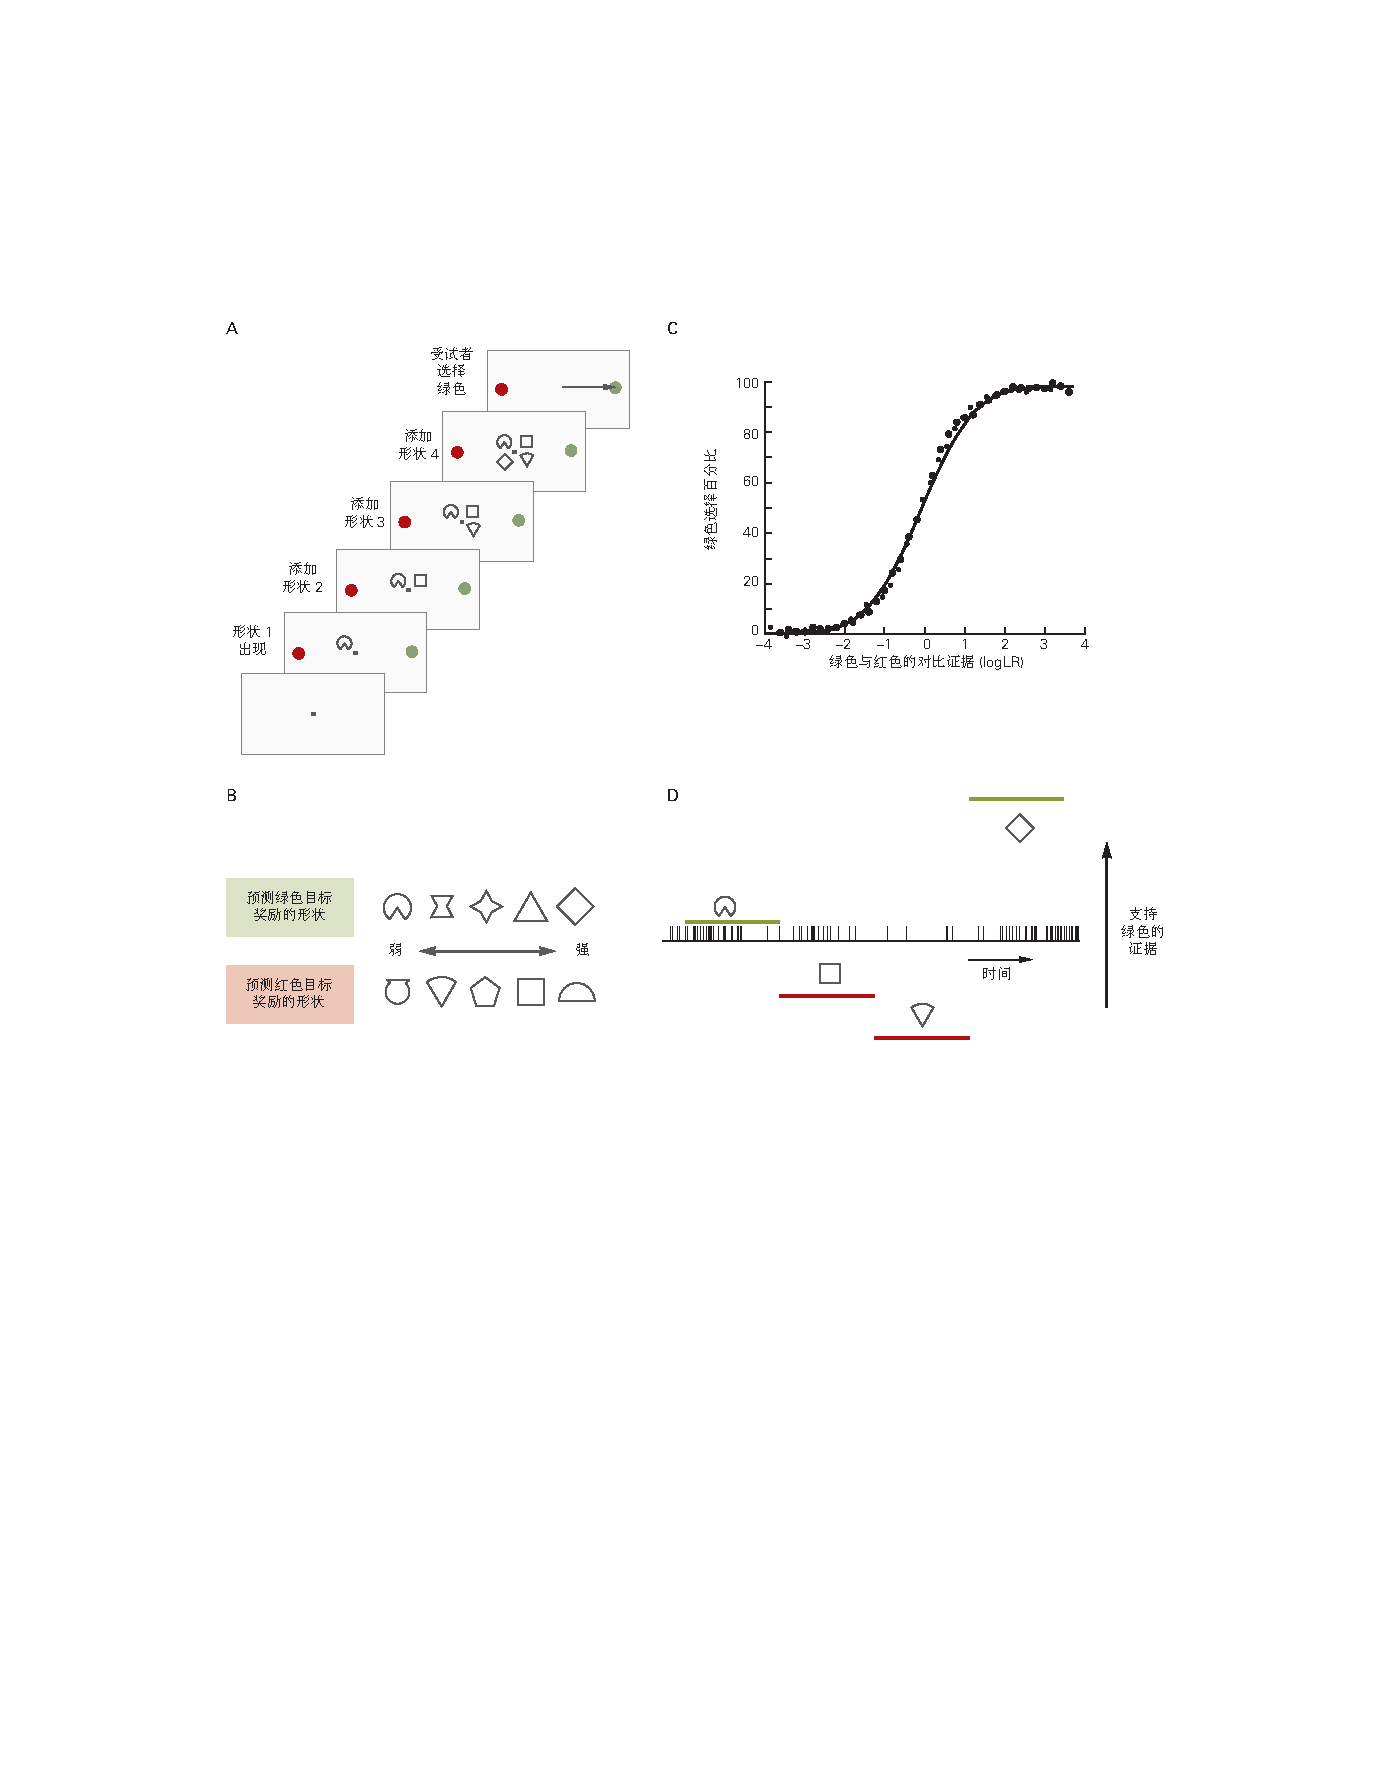
\includegraphics[width=1.0\linewidth]{chap56/fig_56_9}
	\caption{证据积累是从证据符号进行概率推理的基础。
		\textbf{A.} 一只猴子被训练根据四个形状的序列做出决定,从一组 10 个形状中随机抽取并替换。
		这些形状每半秒按顺序添加到显示中。
		\textbf{B.} 每个形状提供不同数量的证据表明奖励与红色或绿色选择目标相关联。
		有些,如菱形和半圆,是高度可靠的预测指标,如果分别选择绿色或红色,就会出现奖励。
		其他人则不太可靠。 可靠性的程度由似然比或其对数来量化。
		一个好的决策者应该根据似然比的乘积或其对数之和(\textit{对数似然比})做出决策。
		\textbf{C.} 猴子的决定是由四种形状的概率证据指导的。
		在四种形状的\textit{对数似然比}之和强烈偏爱绿色的试验中,猴子几乎总是选择绿色。
		当总和接近于 0 时,猴子不得不根据薄弱的证据做出决定,并做出不那么一致的选择。
		选择的模式表明,猴子将更大的权重分配给更可靠的形状(强与弱)。
		\textbf{D.} 在知觉决策任务中研究的相同类型的顶叶神经元代表了在其反应域中与选择目标有关的证据的运行总和。
		当绿色目标位于神经元的响应区域中时,单个决策会显示尖峰。
		尖峰下方的水平黑线标志着绿色与红色证据的中性水平,这样两个选择目标获得奖励的可能性相同。
		与指示形状的每个连续呈现相关联的绿线或红线的垂直位置显示了奖励在绿色目标处的形状所赋予的累积证据。
		第一个形状是绿色的微弱证据。
		第二和第三个形状提供了越来越多的反对绿色(红色)的证据。 注意射速的降低。
		最终的形状为绿色提供了强有力的证据,因此所有形状的累积证据都偏向于绿色。
		注意射速的增加。
		它是联合皮层中单个神经元使用持续活动来计算对决策有用的数量的示例。
		根据许多试验的放电率,结果表明神经元编码概率比对数的累积和-奖励与神经元响应域中的选择目标相关联的\textit{对数似然比}\cite{yang2007probabilistic}。}
	\label{fig:56_9}
\end{figure}


当猴子做出决定时,在运动任务中研究的同一顶叶区域记录了神经活动。
和以前一样,神经元的反应方式揭示了在其反应场中形成支持或反对选择目标的决定。
当红色目标位于反应场中时,神经元将正值分配给偏爱红色的形状,将负值分配给偏爱绿色的形状。
当绿色目标在响应字段中时,符号相反。
如示例所示,当呈现四种形状中的每一种时,响应会发生离散变化,并且变化量与可靠性程度相称。
事实上,增量(或减量)与实验者分配给形状的 \textit{对数似然比}成正比!
大脑只是简单地将这些\textit{对数似然比}相加以形成一个决定。
如果允许猴子查看任意数量的形状,它通常会在累积的证据(以\textit{对数似然比}为单位)达到标准水平时停止。
\textit{侧顶叶}神经元做与它们在运动决策中所做的相同的事情。
它们产生的发射率表示噪声增量和减量的累积和。


通过添加\textit{对数似然比}单位,大脑以统计学家或精算师结合来自多个来源的证据的方式从概率线索中实现推理。
实验表明,用于感知决策的机制也在更复杂的决策中发挥作用,这些决策涉及从更抽象的证据来源进行推理。
它涉及本章更广泛的主题:
对决策的研究提供了对大脑如何实现各种认知功能的洞察力。



\section{偏好决策使用了关于价值的证据}

许多(如果不是大多数的话)人类和动物做出的决定都是基于价值分配的偏好表达。 
在某些情况下,价值是与生俱来的。
例如,大多数动物对甜的体验是积极的,对苦的体验是消极的(第~\ref{chap:chap29}~章)。
然而,在绝大多数情况下,价值是通过经验获得的,或者是从基于其他偏好的推理中得出的。
与关于运动方向、医学诊断或天气的决定不同,关于一个人更喜欢一对物品中的哪一个的决定在客观上不是正确的或错误的。
只能说是符合或不符合一个人的价值表达。
事实上,我们对主体对客体评价的了解只能通过观察她的选择来揭示给我们。


然而,尽管主观证据和客观证据之间存在质的差异,但支持感知和基于价值的决策的神经机制之间存在相似之处。
与价值相差很大的项目相比,决策者在具有相似价值的项目之间进行选择需要花费更多的时间,而且他们的选择也不那么一致。
在一个典型的实验中,参与者被要求指出他们稍后将做出选择的每个项目的价值。
例如,他们可能会被问到他们愿意支付多少,或者他们被要求给出从非常不受欢迎到中性再到非常理想的评级。
通常重复此过程以为要在实验中使用的每个项目提供主观值。


然后要求参与者在成对的项目之间做出决定。
实验前传达的主观价值观的差异提供了项目之间决策难度的指标。
它类似于运动相干性。
类似的方法适用于动物。
例如,一只猴子可能会表现出更喜欢葡萄汁而不是苹果汁,然后被要求在少量葡萄汁和大量苹果汁之间做出选择。
通过滴定体积与导致猴子以相同倾向选择任一果汁的值的比率,该决定变得更加困难。


已经确定了与这种类型的值编码相关的两种类型的神经元。
第一个通常位于纹状体中,编码与动作相关的值。
第二个,主要在眶额和扣带皮层,似乎对与特定项目相关的价值进行编码。
关于偏好的决定似乎来自支配知觉决定的相同策略。
正如左右运动的决定是由左右偏好的感觉神经元的放电率差异决定的,两个项目之间的决定是基于编码每个项目值的神经元活动的差异。
这些神经表征是嘈杂的,这个特征可以解释为什么决策者可能会做出与其价值观不一致的选择。
这也可以解释为什么在具有相似价值的项目之间做出决策往往需要更多时间,类似于上面讨论的速度-准确性权衡的速度-一致性权衡。


与感性决策的类比很吸引人,但它忽略了基于价值的决策更有趣的方面。
如上所述,大多数物品的价值不是生物学赋予的,而是后天习得的。
此外,没有理由假设这种价值是单价的。
人们可能会根据不同的品质和考虑因素对一件物品进行不同的估价,并且在不同的情况下,其中一种或多种品质可能占主导地位。
因此,一个项目的价值可能会仅仅因为与另一个项目进行比较而发生变化,这可能会引起对或多或少令人满意的方面的强调。
新颖性、熟悉性和探索本身的价值也可能在修正主观评价中发挥作用。


这些考虑可能会导致价值的“嘈杂”表示,这被认为可以解释偏好选择中的不一致和较长的决策时间。
这种类型的噪声掩盖了比随机点显示的可变性和神经元的噪声尖峰率复杂得多的过程。
这种评价过程可能涉及前瞻和记忆检索,这在神经水平上才刚刚开始被理解(第~\ref{chap:chap52}~章)。
最后,这些过程必须提供与物品的相对价值有关的证据样本,这些证据要么被积累,要么根据标准单独评估,以决定停止该过程。



\section{决策为理解思维过程、认知状态和意识状态提供了一个框架}

知识状态具有持久性。 即使它们涉及来自感官的信息,感觉知识通常比感觉活动本身更持久。
通过这种方式,知识状态类似于知觉决定,基于感官证据对关于目标的命题的承诺。
正如我们所见,这些状态通常与可能的行为有关,而不是与感官信息的特征有关。
这是许多哲学家和心理学家\textit{詹姆斯$\cdot$吉布森}所主张的立场。


这个简单的观点可以根据经验得出。
持续的神经活动不会出现在大脑的感觉区域,除非刺激是不变的,并且只有当神经元不适应时。
自然地,感觉神经元必须在环境变化或观察者在环境中移动时改变它们的反应,而知识状态通过感觉变化持续存在并且没有连续的输入流。
事实上,在将信息来源(来自感官和记忆)与组织行为的回路相关联的大脑区域中,持续活动是显而易见的。


在前额叶皮层,持续状态代表行动计划、抽象规则和策略。
在顶叶和颞叶中,神经表征具有知识和知识所依赖的行为的双重特征,例如眼球运动或伸手、进食或躲避。
如果投影的目标是眼球运动系统,则响应可以类似于空间表示,就像它们在\textit{侧顶叶}区域中所做的那样,但这只是因为空间和动作之间存在对应关系。
一个有用的指南是考虑关联的来源和目标。
如果源是视觉皮层,目标是控制手部姿势(例如,抓握)的运动前区,就像它们在顶内前区所做的那样(图~\ref{fig:56_7}C),则关联区域可能传达有关曲率、距离、凸度的知识, 和质地。
人们可能倾向于使用从几何学借来的术语来对这些知识进行分类,但考虑有机体可用的手形库可能更简单。
重要的是,联合皮层中的神经元不会立即采取行动。
它们代表以某种方式行事的可能性:意图或临时可供性(方框~\ref{box:56_1})。


\begin{proposition}[启示、感知和知识] \label{box:56_1}
	
	\quad \quad \textit{詹姆斯$\cdot$吉布森}以其感知生态学理论而闻名,他将可承受性称为物体和环境的属性。
	这个词来自动词“负担得起”。
	目标提供了可能的行为,例如抬起,抓取,填充,隐藏,在(例如羊皮纸)或(例如刷子)上绘制/书写或行走。
	可承受性是指动物的潜在行为。同样的物体,比如石头,可以抓取、掉落、破碎(即用作工具)、投掷(作为导弹武器)或钉住(作为镇纸)。
	
	\quad \quad 吉布森因声称感知过程直接从光学阵列中获得这些启示而受到广泛批评,他称之为“直接感知”。
	这个术语通常被误解为与信息处理的计算账户相反。
	通过“直接感知”,吉布森并不意味着对通过感官接收到的数据没有计算。他促进了对这些运算的数学理解。
	他的意思是我们不感知中间物。
	
	\quad \quad 我们确实能感知到物体被视线中的物体意外遮挡的部分,我们也能感知到不透明物体的背面被其正面遮挡。
	我们看不到轮廓、线条艺术和许多其他细节,但这并不是说它们不在视网膜和视觉皮层上。
	吉布森认为,视觉信息的表征并不是感知的充分条件。
	从决策神经科学的角度来看,人们可能会强调潜在行为的表现,比如对计划的临时承诺。
	
	\quad \quad 可承受性仍然是指一类动作,但它是关于动作(例如投掷)或策略的组织,也不一定是物体的质量。
	修饰语“临时”强调该动作可能现在或将来都不会发生。
	这个修饰语在吉布森使用“可承受性”一词时是多余的,因为可承受性是物体的属性(在他的生态框架中),因此具有独立于感知者的永久性。
	
\end{proposition}


让我们暂时搁置知识状态的方面,包括有意识的意识,并将更简单的知识感视为一种可能的利用状态。
这种前意识的想法可能是动物与环境互动的主要状态。
它也可以说是人类经验的最大份额,尽管因为我们没有意识到它,我们低估了它的主导地位。
从这个角度可以得出两个重要的见解。
首先是知识和神经元活动之间的对应关系存在于感觉和行为之间的大脑组织水平上。
尽管来自感觉上皮细胞(例如,视网膜)的信息流通过初级皮层感觉区对于感知至关重要,但高层大脑区域活动产生的知识具有时间灵活性和持久性,这在低层大脑区域是看不到的,哲学家\textit{莫里斯$\cdot$梅洛-庞蒂}称现在的时间厚度。


第二个见解是,导致知识状态的计算具有决策结构,对某种近似于行为库子菜单中可能选择的事物的临时承诺。
我们可以说,顶叶联合神经元会询问感觉区域,以寻找与行为可能性相关的证据:看那里,伸手去拿,以这种方式握住手。
当然,神经元不会提问。
尽管如此,我们还是可以将回路想象成它们在扫描世界,寻找与可能行为有关的证据。
他们可以访问的信息类型受到功能和解剖连接的限制。
问题的类型由投影的目标构成,例如控制凝视、伸手和抓握的区域。


亚瑟柯南道尔爵士赋予夏洛克福尔摩斯这样的洞察力,即发现的关键是知道在哪里寻找以及寻找什么。
我们通过控制大脑的询问系统来获取知识。
有些审讯是自动的,而另一些则是习得的。
前者的一个例子是视野中物体亮度的突然变化;
它提供了有关将眼睛或身体朝向它的可能性的证据。
后者的一个例子是学习和觅食;
我们通过游戏和社交互动(例如,学校)学习如何寻找隐藏的物品以及如何以有目标的方式进行探索。


这种结构的美妙之处在于,问题的答案赋予了一种意义。
即使对于像“我可以看那里吗?”这样平凡的问题,一个肯定的答案,即决定(可能)在一个人的视野外围看一个尚未定义的物体,赋予了关于该项目的空间知识。
在我们直接观察它以识别它是什么之前,我们知道它的存在。
从决策的角度来看,物体的位置是不被感知的,因为在视野的地图中存在神经活动。
相反,位置被感知是因为视野的某些方面(对比度的斑点、亮度的变化、外观或消失),肯定地回答了上述问题。


这种思维方式有助于我们理解术语“失认”所知道的疾病状态,该词来自希腊语,意思是“缺乏知识”。
典型的例子是视觉偏视,这是由顶叶损伤引起的(第~\ref{chap:chap59}~章)。
右顶叶损伤的患者会忽略视野的左侧以及物体的左侧,即使整个物体都在右侧视野中(图~\ref{fig:56_10};另请参见图~\ref{fig:59_1})。
不同于左侧盲,称为同向偏盲(或半盲),它伴随着右侧视觉皮层的损伤(同向是因为无论使用哪只眼睛都是一样的),患有顶叶病变的患者不会抱怨无法看。
她没有意识到赤字,以至于过马路是一个重大危险。


\begin{figure}[htbp]
	\centering
	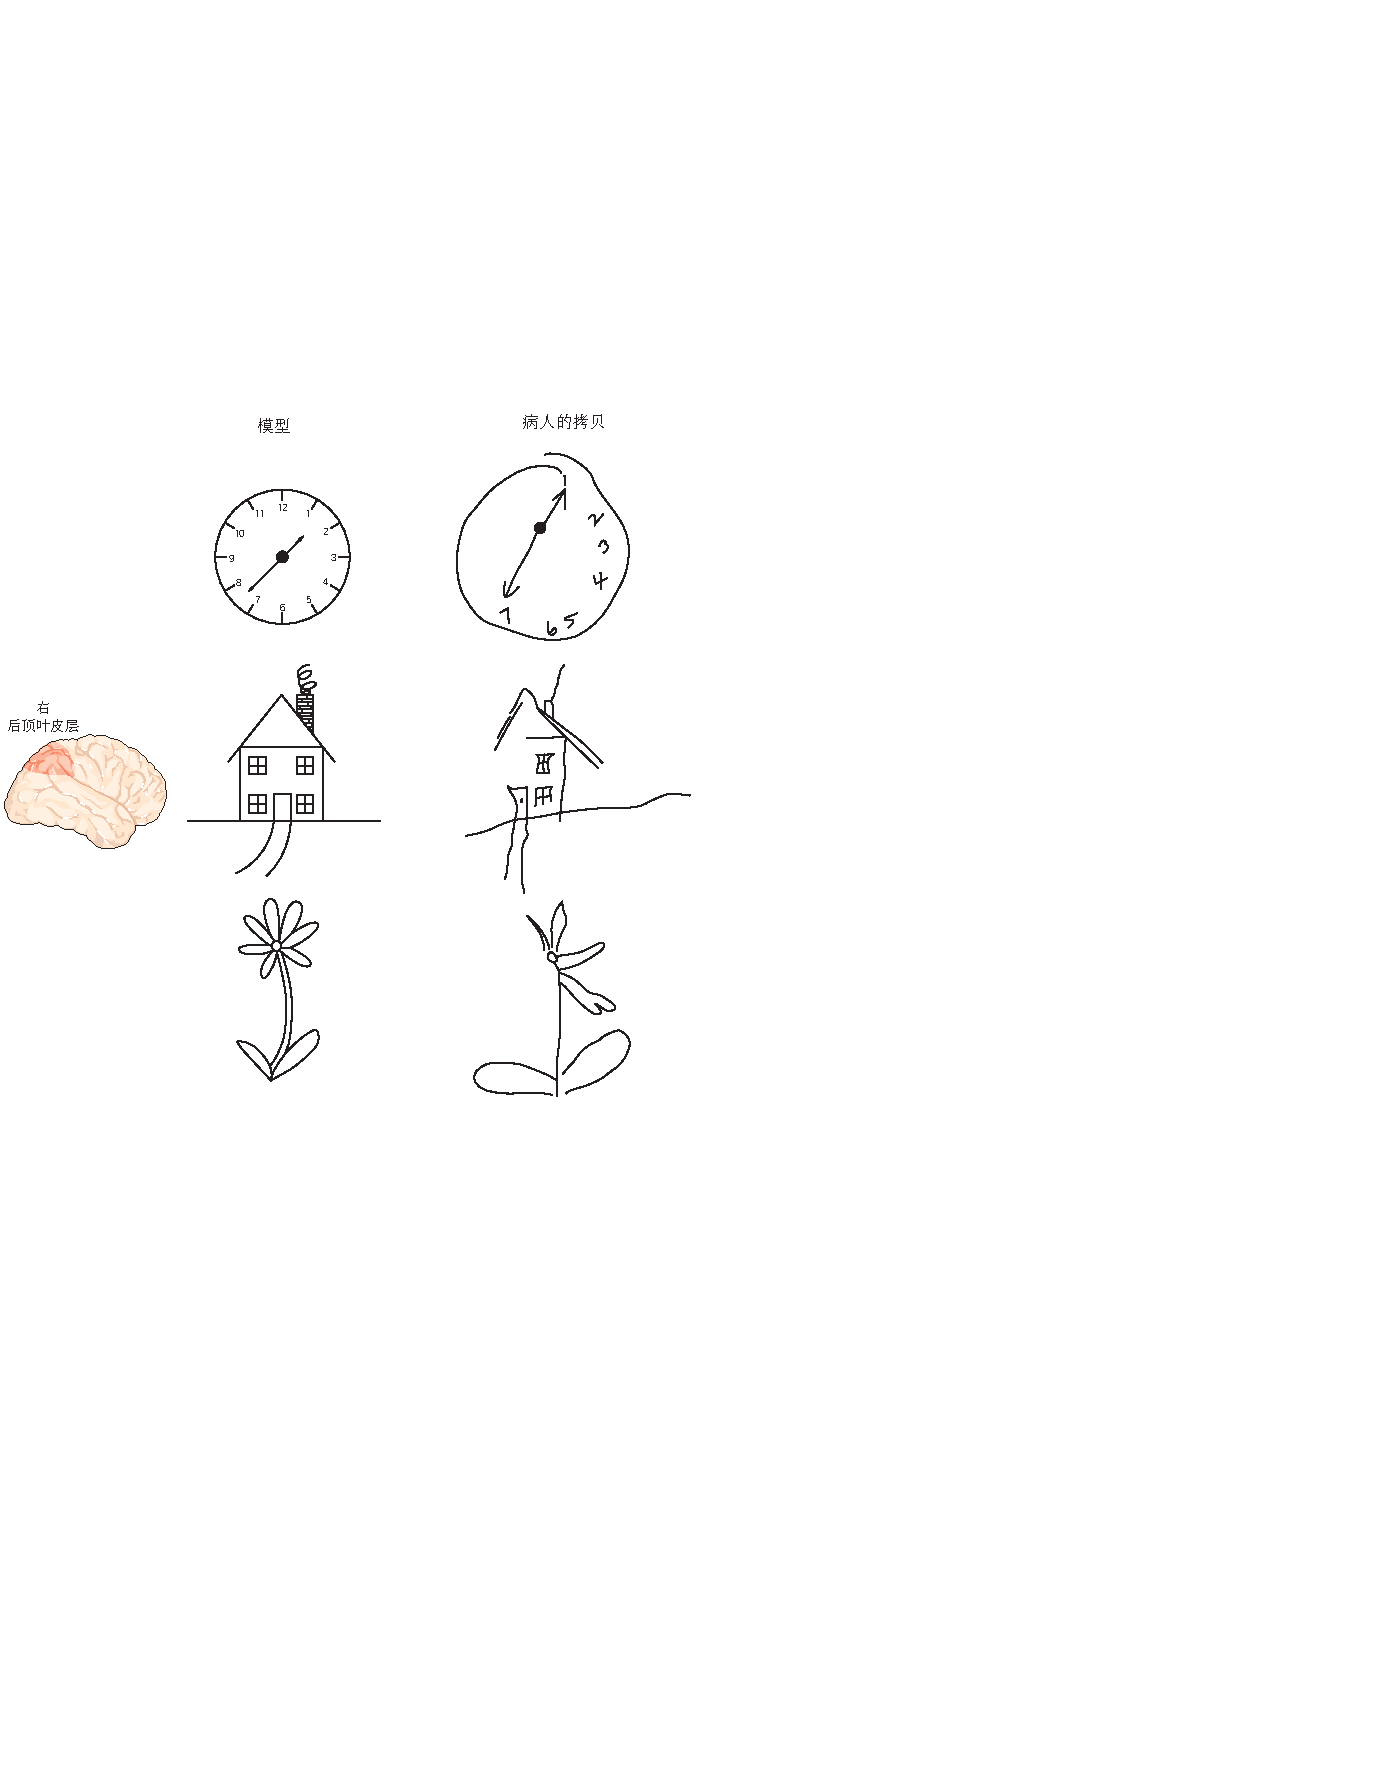
\includegraphics[width=0.83\linewidth]{chap56/fig_56_10}
	\caption{顶叶或颞叶皮层受损会导致失认症或认知缺陷。
		右顶叶受损后,许多患者意识不到左侧空间或物体的左侧部分。
		右图为右后顶叶皮层损伤后单侧视忽视患者所绘。
		通过转移注意力也可以在健康个体中诱发失认症(见图~\ref{fig:25_8})。}
	\label{fig:56_10}
\end{figure}


右视皮层受损的半盲患者仍然期望从左视野询问和接收信息。
当那个病人没有接收到视觉信息时,他知道转身面对与街道平行的方向,从而将其内容放在完整的右半视野中。
相比之下,侧视患者不会首先询问左半场。
她没有感觉到缺少视觉信息,因为进行审讯的设备不工作。
与大多数缺陷一样,大脑(或受损部分)中存在足够的冗余,因此存在一些视觉能力。
事实上,当面对黑暗背景上的单个光点时,即使在受影响的半视野中,同一患者也可能准确地报告光点的存在。


还有其他版本的\textit{偏侧忽略症}涉及缺乏对身体的了解。
例如,右顶骨受伤的患者可能否认她的左臂是她的。
她可能认出那是一只手臂,但否认那是她的。
当被问到这是谁的手臂时,她可能会表示无知近乎冷漠(个人经验)。
该综合症通常还伴有一些视觉忽视以及身体同侧的一些虚弱,这表明更靠头侧和更优越的定位。
考虑到我们部分通过体感系统了解身体的位置,部分通过我们的运动命令的预测结果,部分通过视觉。
手臂尤其是我们较低视野的一个共同特征。
确实,我们习惯于忽略它。


这些例子是最常见的失认症(谢天谢地很少见)。
其他众所周知的例子涉及面部识别(面部失认症)和颜色感知(全色盲)问题,两者都与颞叶病变有关。
不同类型的失认症与我们在第~\ref{chap:chap24}~章中学到的解剖学专业有松散的对应关系。
特别是,中央视觉通路腹侧延伸到颞叶被称为\textit{内容通路},它包含专门的回路 用于处理面孔、物体、颜色和语义记忆。
被称为\textit{空间通路}或“如何”通路的背侧延伸似乎与支持定位的表征有关。


另一种表述将根据与行为相关目标的关联来描述这些流。
对于背侧流,那些是顶叶区域,它们投射到伸手、看或抓握的运动系统。
对于腹侧流,这些是颞叶区域,其投射到指导觅食决定进食、避免、隐藏、接近、交配和交流的结构。
最后几种行为是由颜色和面部特征/表情赋予的社会可供性。
稍加想象,社会可供性的组织与人类颞叶(和颞顶叶交界处)的其他功能相关联。
例如,这些区域与语言理解和推断他人的想法有关。
前者与毁灭性的失认症有关,称为\textit{韦尼克}失语症(第~\ref{chap:chap1}~章和第~\ref{chap:chap55}~章);
后者被称为心理理论,将在下面讨论。


从决策的角度来看,感知、相信和思考具有对命题的临时承诺的性质。
与知觉(无论是感知还是相信)相对应的大脑状态与决策有两个重要方面:经得起感觉和运动流变化的扩展时间特征(即不受即时影响)和命题特征被术语“可供性”所捕获。
知道不仅仅是关于信息,而且就像决定接受一个命题的结果:
我可以做某事,制定某事,接近某人,还是保留尝试我现在不选择的选项的可能性?


有两个警告值得一提。
该框架不会取代信息处理的计算帐户,也不会解释支持这些计算的神经机制。
它主要告诉我们执行这些操作的大脑组织水平。
例如,考虑寻找获得关于红色知识的神经元,尽管早晨和傍晚的光的光谱含量发生变化,这种现象称为颜色恒常性。
与其在感觉区域中寻找以这种不变方式对红色有选择性反应的神经元,不如寻找指导选择成熟水果的神经元。
尽管照明光的光谱含量有所变化,但这并没有避免恢复水果表皮的表面反射特性所需的计算。
用于此类计算的原始数据由感觉神经元提供,这些神经元缺乏颜色恒常性并随着环境的变化保持时间保真度。
然而,知识状态“红色”对于光源是不变的并且可能是持久的。
在缺乏语言的动物中,知识状态可能无法与“成熟的植物”分离。


第二个警告是我们没有区分我们有意识地意识到的知识状态和我们无意识地体验到的知识状态。
例如,当我穿过森林试图找到我听到潺潺流水声的小溪时,我的大脑可能会考虑我经过的物体的位置,这些物体是可抓握的、附着在植被上的,并且颜色表明已经成熟。
我可能有意识地没有意识到这一点。
然而,在我寻找食物的那天晚上,我可能会在这些无意识的遭遇的指引下回到森林的这一部分。
我可能会这样做而不知道为什么,或者记忆可能会刺穿意识。
到目前为止所说的一切都适用于有意识和无意识的体验。我们现在准备阐明差异。



\section{意识可以通过决策的镜头来理解}

显然,我们没有意识到大脑中发生的大部分操作,即使对于最终刺穿意识的过程也是如此。
这就是为什么弗洛伊德著名地讽刺意识被高估了。
进入我们意识的每一个想法都始于对该想法的有意识意识之前的神经计算。
事实上,无意识心理过程的复杂性,包括那些导致“我明白了!”的心理过程。
我们在接听电话时进行的时刻和活动涉及在没有意识的情况下做出的决定。


研究无意识处理是困难的,因为人们否认该过程的经验。
事实上,无意识体验这个词似乎是一个矛盾修辞法。
实验者必须找到一种方法来证明尽管受试者没有意识到信息处理已经发生。
近年来,已经有可能建立条件,从而向人类主体提供信息,这些信息很可能被忽视但仍然能够影响行为,从而允许对无意识心理过程进行科学表征(第~\ref{chap:chap59}~章)。
这鼓励了神经科学家去探究引起思想、知觉和运动的神经活动是什么,这些思想、知觉和运动确实达到了有意识的意识。
我们不会在这里回顾这个庞大的话题,而是分享一个中肯的见解:
从决策的角度来看,意识问题可能比想象的要简单。


从广义上讲,两组现象属于意识标题。
第一个涉及觉醒水平。
一个人在睡着、全身麻醉、昏迷或全身性癫痫发作时没有意识。
一个人在清醒时是完全有意识的,并且在这些极端之间存在意识水平。
这些状态与混乱、解离、昏迷和迟钝等术语相关。
一些意识改变是正常的(例如,睡眠),而其他意识改变是由毒素(例如,酒精)、代谢紊乱(例如,低血糖)、低氧、外伤(例如,脑震荡)或发烧(例如,谵妄)引起的。


这些状态背后的神经科学(以及它们之间的转变)对医学来说非常重要。
我们可以将这组现象归类为神经学意识。
然而,当大多数人谈到意识的奥秘时,这些话题并不是他们的意思。
这部分是因为它们不那么神秘,但也因为它们的特征更客观,而且可以在动物身上研究这些现象。
也就是说,关于负责睡眠、觉醒、麻醉等的机制还有很多需要了解的地方。
许多神经科学正在快速展开(第~\ref{chap:chap44}~章)。


我们不会在这里多说神经学意识,只是为了播种一种有用的见解。
想象一下,当户外暴风雨袭来时,一对母亲和父亲在他们的卧室里睡得很舒服。
还有交通声音,甚至偶尔有雷声。
这一幕持续了一段时间,直到婴儿的哭声惊醒了父母。
这种常见现象告诉我们,无意识的大脑能够处理声音并决定变得有意识。
它无意识地决定,一些声音提供了更多睡眠的机会,而另一些声音则发出了养育的呼唤。
这个决定类似于本章前面考虑的感知决定。 两者都涉及对证据的无意识处理。
然而,唤醒和父母的承诺是有意识地参与环境的决定。
这可能是神经学意识和你在阅读这些文字时所体验到的更有趣的意识之间的试金石(或者作者希望如此)。


当神经科学家、心理学家和哲学家思考意识的奥秘时,他们指的是比清醒更崇高的主题。
这组更高层次的现象包括意识、意象、意志和能动性。
所有有意识的体验都有主观成分。
有意识的感知体验包含了一种感觉,即是我在看内容。
它在意志上与“我”平行。
并不是我的手臂自己动了;
我让它动了!
我们在本章前面使用了“深思熟虑”一词来描述导致决策的思维过程。
我们对这个词的使用是隐喻性的。
它描述了计算和生物机制,但不需要意识。
实际的深思熟虑意味着有意识的意图。
我们知道沿途的推理步骤。
如果我们被问到,我们可以报告我们所依赖的证据,即我们在决策过程中有意识地意识到的证据,以及我们可能无意识地使用的一些证据,如果它们可以从记忆中获取并包含在我们的报告中。
对一个项目的有意识意识和对该项目的无意识处理之间的区别是否仅仅是大脑是否决定了报告的可能性?
能这么简单吗?


考虑以下场景。
一位心理学家得出结论,研究参与者无意识地看到了一些东西,因为该项目影响了后续行为,而参与者否认看到了它。
假设随后的行为涉及向目标的方向伸手。
根据我们对决策的了解,我们可以得出结论,像前面讨论的那样的大脑回路收到了足够的证据来确定看、伸手和接近的可能性,但没有足够的证据来确定报告的可能性。
正如大脑接受看、伸手或抓住的可能性一样,它也可能接受报告的可能性。
也就是说,报告也是一种临时的可供性。


事件提供了报告的可能性,这包括通过决策获得的知识的无意识状态。
事实上,做出决定的事件可能是有意识地体验到的(顿悟时刻)通过另一个报告的决定。
在研究场景中,参与者没有意识到该项目,因为她的大脑没有提交临时报告。
证据不满足决策标准,例如本章前面考虑的感知决策任务中的终止界限。


这个描述为参与者未能报告她看到了该项目提供了一个合理的解释,但仅仅娱乐报告的可能性似乎并不能解释知觉体验本身的现象学,至少乍一看不能。
这种解释需要更仔细地考虑报告的性质。
正如我们将空间知识状态附加到用于伸手和抓取的手的配置上一样,我们必须考虑伴随报告可供性的知识状态。
无论是通过语言还是手势(例如,指向),报告都是与一个代理人或自己(例如,在未来)的临时交流。
它假定了解接收者的思想。


认知科学家使用术语心理理论来指代这种类型的知识或心智能力。
它可以通过要求某人推理另一个代理人行为背后的动机来证明,并且可以通过检查他们对另一个孩子或木偶的反应来研究动物和不会说话的儿童。
在一项研究方案中,两名儿童见证了一个想要的玩具被放在左侧或右侧的容器中(图~\ref{fig:62_2})。
然后,当另一个孩子不在时,测试儿童会目睹玩具移动到另一个容器中。
当那个孩子回来时,实验者评估测试孩子对返回的孩子将打开哪个容器找到玩具的期望。
3 岁以下的儿童不会通过该测定表现出心智理论。
他们认为返回的孩子会打开装有玩具的容器,而不是转移前的容器。
人类以外的动物是否有心理理论是有争议的。
我们怀疑在动物界和 3 岁以下的儿童中存在这种能力的早期形式。
当成年人执行依赖于心智理论的任务时,右颞顶叶交界处和\textit{颞上沟}是活跃的。


心理理论(与叙述相结合)对与报告可供性相关的知识状态具有深远的影响。
想象一下,一个女人正在看着放在桌子上的电钻。
她体验了钻头相对于她的眼睛和手的位置,以及它的质地和形状。
它有一个可抓握的表面,部分在她的视线范围内,部分被遮挡(例如,背部)。
这些是通过临时承诺查看、伸手和掌握演习而产生的知识状态。
它们可能涉及类似于图~\ref{fig:56_7}~中所示的神经活动,并且它们是简单决策的结果。
钻头让人想起与其作为工具的效用相关的其他可供性,它可能产生噪音,以及一端锋利的钻头带来的潜在危险。
这是一个精心制作的、潜在丰富的知识集合,但它可以在无意识中体验到。
例如,如果该女性全神贯注于其他任务,例如与朋友通电话,她可能仍然会利用这些知识状态。


但是假设桌子的另一边有一个男人,假设这个女人(也就是她的大脑)也达成了一个临时承诺,要向这个男人报告他们之间的演习。
考虑她的知识状态的变化。
演习现在不仅出现在她的视野中,相对于她的凝视、她的手和她的动作库,而且出现在男人的视野和他可能的动作中。
据了解,她看不到的钻头部分在该男子的视线范围内。
事实上,她的“心理理论”能力也提供了这样的知识,即演习的其他部分只有她能看到,而且这个男人可能正在体验这些部分,就像她体验不在她直接视线范围内的部分一样,既是前意识地作为对象的被遮挡部分,又是有意识地作为可以从另一个有利位置直接看到的目标的一部分。
演习中有一些东西既是私人的、公共的,又是在世界上的(独立于任何一个人的思想)。
演习是为下一个进入房间的人或想象中的人准备的。
演练知识的转变是从第一人称经验(例如,品质和能力)的集合到世界上拥有自身存在的事物。
可以想象,这种知识状态是我们对世界的有意识意识,或者至少是世界的一部分,因为与报告决定相关的知识状态通过报告本身的内容进一步丰富。


报告可能很简单,比如指出工具或藏身点的位置,也可能涉及叙述。
在隐藏点的情况下,可能会传达额外的内容以表明围栏提供了免受捕食者或捕食者位置的安全。
许多简单的报告不需要叙述,因为诸如工具和围栏之类的物品会持续存在,而心智理论假定工具的可供性或他人头脑中的藏身之处,而事件,也提供了报告的可能性,通常需要叙述,因为它们是 短暂的。


与叙述相关的知识状态可以包含历史、模拟、预测、病因学(例如,起源故事)、目的和结果。
对于演习,叙述可能会增强知识状态,包括购买地点的记忆、发生故障的情节以及可拆卸钻头的机制。
叙事允许我们在比之前考虑的场景更复杂的环境中进行推理(例如,伞形示例和概率推理任务;图~\ref{fig:56_9})。
如果没有起源故事、模拟、假设、展望和反事实,我们就无法对科学、医学诊断和法理学进行推理。
这种能力的进化优势是显而易见的(至少暂时如此,直到它导致我们让地球无法居住)。


总而言之,当无意识的大脑决定向另一个大脑报告该项目时,可能会出现对该项目的有意识意识。
意图是临时的,因为不需要发生明显的报告(口头或手势),就像顶叶皮层不需要眼球运动来参与可能的注视意图一样。
正如中央凹点的临时意图对应于一个尚未识别的物体在外围的位置的前意识知识,向我们有心理理论的另一个代理人(或自我)报告的可能性对应于一个知识 以一种能满足意识觉察的大部分方面的方式进行。


自然地,我们从感知决策到意识能力的旅程充其量是不完整的。
例如,对于有意识的体验是什么感觉,它还没有提供令人满意的解释。
但这是一个开始,因为它粗略地解释了为什么通过眼睛获得的感官信息与听觉或体感体验不同,它提供了对知觉意识的私人方面以及我们对物体作为事物的体验的洞察。
世界,独立于他们为感知者提供的东西。
这些最后的特征来自另一个代理人的想法。


如果没有别的,从决策的角度来看意识的观点是简化的。
没有理由去寻找赋予意识的大脑特殊区域,或特殊的神经元类型,或信息表示中的特殊成分(例如,振荡或同步),或特殊的机制。
该机制可能看起来像任何其他类型的临时承诺,即一种赋予已知状态但不需要有意识意识的决定。
当然,大脑活动本身并不是有意识的,就像支持可能的手势的大脑活动不是手势本身一样。
从这个意义上说,意识机制与其他可供性的唯一不同之处在于它涉及报告而不是到达、看向、吃、喝、躲藏、穿过和交配。
所有这些都可能涉及决策形成和阈值检测。


因此,通过研究决策的神经科学,我们也在研究意识的神经科学。
关于本章第一部分中描述的最简单决策的机制,还有很多东西需要学习。
例如,我们不知道是什么设定了界限,也不知道阈值是如何在大脑回路中实现的。
然而,这些和其他基本问题的答案是现代神经科学的目标,因此,人类意识也是如此。



\section{亮点}

1. 决策是基于证据、先验知识和预期结果对提议、行动或计划的承诺(在选项中)。
该承诺不需要立即采取行动或任何行为,并且可以修改。 


2. 决策为认知神经科学提供了一个窗口。
它模拟了不受感官处理和身体肌肉组织控制的直接需求影响的偶然行为和心理操作。


3. 通过对与备选方案有关的证据状态应用规则来形成决定。
在两个备选方案之间进行选择的简单决策规则采用了一个标准。
如果证据超出标准,则选择证据支持的备选方案;
如果不是,请选择其他选项。


4. 对于某些知觉决策,证据来源及其神经表征是已知的。


5. 许多决策的准确性受到信号强度及其相关噪声的限制。
对于神经系统,这种噪声归因于单个神经元的可变放电,因此代表证据的少量神经元的可变放电率。


6. 许多决策受益于跨时间组合的多个证据样本。
这样的决策过程需要时间,并且需要能够保存和更新累积证据(即决策变量)的神经表征。
前额叶和顶叶皮层中的神经元能够保持和更新它们的放电率,代表不断变化的决策变量。
这些神经元还参与计划、注意力和工作记忆。


7. 速度-准确性的权衡是通过对终止决定所需的证据数量设定界限或阈值来控制的。
这是使一个决策者与众不同的政策示例。


8. 许多决定是关于对有机体具有不同价值的命题、项目或目标。
这种基于价值的决策取决于项目和效价之间存储的关联。 


9. 许多决定的证据来源是记忆和对环境的主动审问(信息搜寻)。
当动物觅食和探索时,以及当爵士音乐家即兴创作时,这些操作就会发挥作用。


10. 决策让我们不再将知识视为神经表征的涌现属性,而是对与命题、计划和可供性有关的证据进行定向的、主要是无意识的询问的结果。
意图是临时的,因为不需要采取公开的行动。
正如中央凹点的临时意图对应于一个尚未识别的物体在外围的位置的前意识知识,向我们有心理理论的另一个代理人(或自我)报告的可能性对应于一个知识 项目以我们有意识地意识到它的方式。


11. 从决策的角度来看,当无意识的大脑做出向另一个大脑报告的决定时,可能会出现对某个项目的有意识意识。
可供性具有叙述的性质,很像无声的言语或先于语言表达的想法。
它还使物体在其他思想所居住的环境中存在,因此独立于感知者的思想。
它将私人和公共内容赋予所感知的目标的各个方面。


